\documentclass[12pt,a4paper]{article}

% --- Essential Packages ---
\usepackage[utf8]{inputenc}
\usepackage[T1]{fontenc}
\usepackage{mathptmx} % Times Roman typography
\usepackage[a4paper, left=24mm, right=24mm, top=24mm, bottom=25mm]{geometry}
\usepackage{graphicx}
\usepackage[table,svgnames,dvipsnames]{xcolor}
\usepackage{amsmath, amssymb}
\usepackage{setspace}
\usepackage{enumitem}
\usepackage{array}
\usepackage{tabularx}
\usepackage{booktabs}
\usepackage{listings}
\usepackage{tikz}
\usepackage{eso-pic}
\usepackage{fancyhdr}
\usepackage{hyperref}

% --- Custom Colors ---
\definecolor{darkred}{RGB}{140, 20, 20}
\definecolor{navyblue}{RGB}{0, 32, 96}

% --- Hyperref Setup ---
\hypersetup{
    colorlinks=true,
    linkcolor=black,
    filecolor=navyblue,
    urlcolor=blue,
    citecolor=darkred,
    pdftitle={DESIGN AND FABRICATION OF PARABOLIC WATER HEATER WITH SOLAR TRACKING AND POWER GENERATION},
    pdfauthor={Government Polytechnic Amravati - Department of Mechanical Engineering}
}

% --- Code Listing Styling for Arduino C++ ---
\lstset{
    language=C++,
    basicstyle=\fontsize{9.5}{13}\ttfamily,
    keywordstyle=\color{blue}\bfseries,
    stringstyle=\color{red!70!black},
    commentstyle=\color{green!50!black}\itshape,
    numberstyle=\tiny\color{gray},
    numbers=none,
    backgroundcolor=\color{gray!6},
    frame=single,
    rulecolor=\color{gray!50},
    breaklines=true,
    tabsize=2,
    showstringspaces=false
}

% --- Double Border on Every Numbered Content Page ---
\newcommand\DrawDoubleBorder{
  \begin{tikzpicture}[remember picture, overlay]
    \draw[line width=1.5pt, color=black]
      ([xshift=12mm, yshift=-12mm]current page.north west)
      rectangle
      ([xshift=-12mm, yshift=12mm]current page.south east);
    \draw[line width=0.5pt, color=black]
      ([xshift=13.8mm, yshift=-13.8mm]current page.north west)
      rectangle
      ([xshift=-13.8mm, yshift=13.8mm]current page.south east);
  \end{tikzpicture}
}

% --- Page Header and Footer Styling ---
\pagestyle{fancy}
\fancyhf{}
\renewcommand{\headrulewidth}{0pt}
\cfoot{\fontsize{11}{14}\selectfont \textbf{\textasciitilde\ \thepage\ \textasciitilde}}

% Automatically draw double border on every page using fancyhdr
\AddToShipoutPictureBG{%
  \ifnum\value{page}>0
    \ifnum\value{page}<41
      % Preliminary pages (1 to 8 in PDF have page counter <= 0 or empty pagestyle)
    \fi
  \fi
}

\begin{document}

% ==============================================================================
% MODULAR PAGE INCLUSIONS (PAGES 1 TO 48)
% ==============================================================================

% --- Page 1 ---
% ==============================================================================
% PAGE 1: OUTER COVER PAGE
% ==============================================================================
\thispagestyle{empty}
\begin{tikzpicture}[remember picture, overlay]
  % Dark background
  \fill[fill=black!92] (current page.north west) rectangle (current page.south east);
  % Outer Gold Border
  \draw[line width=2.5pt, color=Goldenrod!90!black]
    ([xshift=12mm, yshift=-12mm]current page.north west) rectangle ([xshift=-12mm, yshift=12mm]current page.south east);
  % Inner Gold Border
  \draw[line width=1.0pt, color=Goldenrod!80!black]
    ([xshift=14.5mm, yshift=-14.5mm]current page.north west) rectangle ([xshift=-14.5mm, yshift=14.5mm]current page.south east);
\end{tikzpicture}

\vspace*{-8mm}
\begin{center}
  {\fontsize{18}{22}\selectfont \bfseries \textcolor{Goldenrod!95!white}{GOVERNMENT POLYTECHNIC,}\\[3mm]
  \textcolor{Goldenrod!95!white}{AMRAVATI}}\\[4mm]
  {\fontsize{10}{13}\selectfont \bfseries \textcolor{Goldenrod!80!white}{(AN AUTONOMOUS INSTITUTE OF GOVERNMENT OF MAHARASHTRA)}}\\[6mm]
  
  
\includegraphics[width=32mm]{figures/gpa_logo.png}\\[6mm]
  
  {\fontsize{13}{16}\selectfont \bfseries \textcolor{Goldenrod!90!white}{DEPARTMENT OF MECHANICAL ENGINEERING}\\[2mm]
  \textcolor{Goldenrod!90!white}{(2025--2026)}}\\[8mm]
  
  {\fontsize{12}{15}\selectfont \bfseries \textcolor{Goldenrod!90!white}{A PROJECT ON}}\\[4mm]
  {\fontsize{13}{17}\selectfont \bfseries \textcolor{Goldenrod!95!white}{``DESIGN AND FABRICATION OF PARABOLIC WATER HEATER\\[2mm]
  WITH SOLAR TRACKING AND POWER GENERATION''}}\\[7mm]
  
  {\fontsize{11}{14}\selectfont \bfseries \textcolor{Goldenrod!90!white}{UNDER THE GUIDANCE OF}}\\[2mm]
  {\fontsize{13}{16}\selectfont \bfseries \underline{\textcolor{Goldenrod!95!white}{Prof. A. R. BANSALI}}}\\[7mm]
  
  {\fontsize{12}{15}\selectfont \bfseries \textcolor{Goldenrod!90!white}{$\sim$SUBMITTED BY$\sim$}}\\[4mm]
  
  \begin{tabular}{ll}
    \textbf{\textcolor{Goldenrod!95!white}{MS. ASHWINI R. HAGE}} & \textbf{\textcolor{Goldenrod!95!white}{(23ME031)}} \\[1.5mm]
    \textbf{\textcolor{Goldenrod!95!white}{MR. ROHAN S. HAGE}}    & \textbf{\textcolor{Goldenrod!95!white}{(23ME032)}} \\[1.5mm]
    \textbf{\textcolor{Goldenrod!95!white}{MR. AMAY P. KADAM}}   & \textbf{\textcolor{Goldenrod!95!white}{(23ME044)}} \\[1.5mm]
    \textbf{\textcolor{Goldenrod!95!white}{MS. NANDINI R. KALE}}  & \textbf{\textcolor{Goldenrod!95!white}{(23ME047)}} \\[1.5mm]
    \textbf{\textcolor{Goldenrod!95!white}{MR. PRANAV V. KALPANDE}} & \textbf{\textcolor{Goldenrod!95!white}{(23ME048)}}
  \end{tabular}
\end{center}
\clearpage


% --- Page 2 ---
% ==============================================================================
% PAGE 2: INNER TITLE / SUBMISSION COVER PAGE
% ==============================================================================
\thispagestyle{empty}
\begin{tikzpicture}[remember picture, overlay]
  \draw[line width=2.0pt, color=Goldenrod!90!black]
    ([xshift=12mm, yshift=-12mm]current page.north west) rectangle ([xshift=-12mm, yshift=12mm]current page.south east);
  \draw[line width=0.8pt, color=Goldenrod!80!black]
    ([xshift=14.5mm, yshift=-14.5mm]current page.north west) rectangle ([xshift=-14.5mm, yshift=14.5mm]current page.south east);
\end{tikzpicture}

\vspace*{-5mm}
\begin{center}
  {\fontsize{18}{22}\selectfont \bfseries \textcolor{darkred}{GOVERNMENT POLYTECHNIC,}\\[2mm]
  \textcolor{darkred}{AMRAVATI}}\\[3mm]
  {\fontsize{10}{13}\selectfont \bfseries (AN AUTONOMOUS INSTITUTE OF GOVERNMENT OF MAHARASHTRA)}\\[5mm]
  
  
\includegraphics[width=30mm]{figures/gpa_logo.png}\\[5mm]
  
  {\fontsize{12}{15}\selectfont \bfseries A PROJECT REPORT ON}\\[4mm]
  {\fontsize{13}{17}\selectfont \bfseries \textcolor{red!75!black}{``DESIGN AND FABRICATION OF PARABOLIC WATER HEATER\\[2mm]
  WITH SOLAR TRACKING AND POWER GENERATION''}}\\[6mm]
  
  {\fontsize{11}{14}\selectfont \bfseries \textcolor{red!75!black}{$\sim$SUBMITTED TO$\sim$}}\\[3mm]
  {\fontsize{14}{18}\selectfont \bfseries GOVERNMENT POLYTECHNIC, AMRAVATI}\\[2mm]
  {\fontsize{9.5}{12.5}\selectfont \bfseries IN PARTIAL FULFILLMENT OF THE REQUIREMENT FOR THE AWARD OF}\\[2mm]
  {\fontsize{13}{16}\selectfont \bfseries DIPLOMA IN MECHANICAL ENGINEERING}\\[6mm]
  
  {\fontsize{11}{14}\selectfont \bfseries $\sim$SUBMITTED BY$\sim$}\\[3.5mm]
  
  \begin{tabular}{ll}
    \textbf{MS. ASHWINI R. HAGE} & \textbf{(23ME031)} \\[1.2mm]
    \textbf{MR. ROHAN S. HAGE}    & \textbf{(23ME032)} \\[1.2mm]
    \textbf{MR. AMAY P. KADAM}   & \textbf{(23ME044)} \\[1.2mm]
    \textbf{MS. NANDINI R. KALE}  & \textbf{(23ME047)} \\[1.2mm]
    \textbf{MR. PRANAV V. KALPANDE} & \textbf{(23ME048)}
  \end{tabular}\\[6mm]
  
  {\fontsize{11}{14}\selectfont \bfseries $\sim$ GUIDED BY $\sim$}\\[2.5mm]
  {\fontsize{13}{16}\selectfont \bfseries \textcolor{darkred}{\underline{Prof. A. R. BANSALI}}}\\[1.5mm]
  {\fontsize{10}{13}\selectfont \bfseries LECTURER IN MECHANICAL ENGINEERING}\\[1mm]
  {\fontsize{10}{13}\selectfont \bfseries GOVERNMENT POLYTECHNIC AMRAVATI}\\[1.5mm]
  {\fontsize{10}{13}\selectfont \bfseries (2025--2026)}
\end{center}
\clearpage


% --- Page 3 ---
% ==============================================================================
% PAGE 3: CERTIFICATE
% ==============================================================================
\thispagestyle{empty}
\begin{tikzpicture}[remember picture, overlay]
  \draw[line width=2.0pt, color=Goldenrod!90!black]
    ([xshift=12mm, yshift=-12mm]current page.north west) rectangle ([xshift=-12mm, yshift=12mm]current page.south east);
  \draw[line width=0.8pt, color=Goldenrod!80!black]
    ([xshift=14.5mm, yshift=-14.5mm]current page.north west) rectangle ([xshift=-14.5mm, yshift=14.5mm]current page.south east);
\end{tikzpicture}

\vspace*{-5mm}
\begin{center}
  {\fontsize{18}{22}\selectfont \bfseries \textcolor{darkred}{GOVERNMENT POLYTECHNIC,}\\[2mm]
  \textcolor{darkred}{AMRAVATI}}\\[3mm]
  {\fontsize{10.5}{13.5}\selectfont (An Autonomous Institute of Government of Maharashtra)}\\[2mm]
  {\fontsize{12}{15}\selectfont \bfseries Department of Mechanical Engineering}\\[4mm]
  
  
\includegraphics[width=28mm]{figures/gpa_logo.png}\\[6mm]
  
  {\fontsize{20}{24}\selectfont \bfseries Certificate}\\[6mm]
\end{center}

\noindent
\begin{spacing}{1.4}
{\fontsize{11.5}{16}\selectfont
This is to certify that, \textbf{Mr. Amay P. Kadam (23ME044)} of $3^{\text{rd}}$ year (Odd term) Diploma in Mechanical Engineering have satisfactorily completed the major project entitled \textbf{\textcolor{red!75!black}{``DESIGN AND FABRICATION OF PARABOLIC WATER HEATER WITH SOLAR TRACKING AND POWER GENERATION''}} of course, \textbf{ME7501- Capstone Project} for the academic year 2025--2026 as prescribed in curriculum.
}
\end{spacing}

\vfill

\begin{table}[h!]
\centering
\begin{tabular*}{\textwidth}{@{\extracolsep{\fill}}cc@{}}
  \textbf{Prof. A. R. Bansali} & \textbf{Prof. S. S. Moon} \\
  Project Guide & Head of Department \\
  (Lecturer in Mechanical Engineering) & (Mechanical Engineering Department)
\end{tabular*}
\end{table}

\vspace{10mm}

\begin{center}
  \textbf{Dr. A. B. Borade}\\[1mm]
  (Principal)\\[1mm]
  (Government polytechnic, Amravati)
\end{center}
\vspace{5mm}
\clearpage


% --- Page 4 ---
% ==============================================================================
% PAGE 4: VISION & MISSION
% ==============================================================================
\thispagestyle{empty}
\begin{tikzpicture}[remember picture, overlay]
  \draw[line width=2.0pt, color=Goldenrod!90!black]
    ([xshift=12mm, yshift=-12mm]current page.north west) rectangle ([xshift=-12mm, yshift=12mm]current page.south east);
  \draw[line width=0.8pt, color=Goldenrod!80!black]
    ([xshift=14.5mm, yshift=-14.5mm]current page.north west) rectangle ([xshift=-14.5mm, yshift=14.5mm]current page.south east);
\end{tikzpicture}

\vspace*{-5mm}
\begin{center}
  {\fontsize{18}{22}\selectfont \bfseries \textcolor{darkred}{GOVERNMENT POLYTECHNIC,}\\[2mm]
  \textcolor{darkred}{AMRAVATI}}\\[3mm]
  {\fontsize{10}{13}\selectfont \bfseries (AN AUTONOMOUS INSTITUTE OF GOVERNMENT OF MAHARASHTRA)}\\[8mm]
  
  {\fontsize{13}{16}\selectfont \bfseries \underline{VISION}}\\[3mm]
\end{center}
\begin{itemize}[leftmargin=12mm, label=\textbullet]
  \item To be a vibrant technical institute of global reputes contributing towards the needs of industries \& society.
\end{itemize}

\begin{center}
  \vspace{4mm}
  {\fontsize{13}{16}\selectfont \bfseries \underline{MISSION}}\\[3mm]
\end{center}
\begin{itemize}[leftmargin=12mm, label=\textbullet]
  \item To develop competent diploma engineers suitable for contemporary industrial environment.
  \item To inculcate socially accepted ethics \& values among budding engineers.
  \item To Nurture innovations and entrepreneurship.
  \item To produce engineers with psychomotor \& cognitive skills committed to lifelong learning.
\end{itemize}

\vspace{8mm}
\begin{center}
  {\fontsize{14}{18}\selectfont \bfseries \textcolor{darkred}{MECHANICAL ENGINEERING DEPARTMENT}}\\[6mm]
  {\fontsize{13}{16}\selectfont \bfseries \underline{VISION}}\\[3mm]
\end{center}
\begin{itemize}[leftmargin=12mm, label=\textbullet]
  \item To become center of excellence in Mechanical Engineering, catering to the needs of industry and society.
\end{itemize}

\begin{center}
  \vspace{4mm}
  {\fontsize{13}{16}\selectfont \bfseries \underline{MISSION}}\\[3mm]
\end{center}
\begin{itemize}[leftmargin=12mm, label=\textbullet]
  \item Provide excellent academic ambience for imparting knowledge and skills.
  \item Inculcate awareness about behavioral skills, ethical practices and sustainable development.
  \item Provide nurturing environment for promoting entrepreneurship.
  \item Respond effectively to the needs of the industry and changing world.
\end{itemize}
\clearpage


% --- Page 5 ---
% ==============================================================================
% PAGE 5: PEOs, POs, PSOs
% ==============================================================================
\thispagestyle{empty}
\begin{tikzpicture}[remember picture, overlay]
  \draw[line width=2.0pt, color=Goldenrod!90!black]
    ([xshift=12mm, yshift=-12mm]current page.north west) rectangle ([xshift=-12mm, yshift=12mm]current page.south east);
  \draw[line width=0.8pt, color=Goldenrod!80!black]
    ([xshift=14.5mm, yshift=-14.5mm]current page.north west) rectangle ([xshift=-14.5mm, yshift=14.5mm]current page.south east);
\end{tikzpicture}

\vspace*{-5mm}
\begin{center}
  {\fontsize{14}{18}\selectfont \bfseries \textcolor{darkred}{MECHANICAL ENGINEERING DEPARTMENT}}\\[4mm]
  {\fontsize{12}{15}\selectfont \bfseries \textcolor{navyblue}{PROGRAMME EDUCATIONAL OBJECTIVES (PEOs)}}\\[2mm]
\end{center}
\noindent
\textbf{PEO1- Technical competence:} Diploma holders will be successful in modern mechanical engineering practice.\\[1.5mm]
\textbf{PEO2- Professional Skills:} Diploma holders will continue to acquire and demonstrate the professional skills necessary to be competent employees or entrepreneurs.\\[1.5mm]
\textbf{PEO3- Professional Attitude and Citizenship:} Diploma holders will become productive and responsible citizens with high ethical and professional standards.

\begin{center}
  \vspace{3mm}
  {\fontsize{12}{15}\selectfont \bfseries \textcolor{navyblue}{PROGRAMME OUTCOMES (POs)}}\\[2mm]
\end{center}
\noindent
\textbf{PO1: Basic and Discipline Specific Knowledge:} Apply knowledge of basic mathematics, science and engineering fundamentals and engineering specialization to solve the engineering problems.\\[1.5mm]
\textbf{PO2: Problem analysis:} Identify and analyze well defined engineering problems using codified standard methods.\\[1.5mm]
\textbf{PO3: Design/development solutions:} Design solutions for well defined technical problems and assists with the design of systems components or processes to meet specified needs.\\[1.5mm]
\textbf{PO4: Engineering tools, Experimentation and testing:} Apply modern engineering tools and appropriate technique to conduct standard tests and measurements.\\[1.5mm]
\textbf{PO5: Engineering practices for Society, sustainability and environment:} Apply appropriate technology in context of society, sustainability, environment and ethical practices.\\[1.5mm]
\textbf{PO6: Project Management:} Use engineering management principles individually, as team member or a leader to manage projects effectively communicate about well-defined engineering activities.\\[1.5mm]
\textbf{PO7: Life-long learning:} Ability to analyze individual needs and engage in updating in the context of technological changes.

\begin{center}
  \vspace{3mm}
  {\fontsize{12}{15}\selectfont \bfseries \textcolor{navyblue}{PROGRAM SPECIFIC OUTCOMES (PSOs):}}\\[2mm]
\end{center}
\noindent
\textbf{PSO1:} To inculcate and foster entrepreneurship.\\[1.5mm]
\textbf{PSO2:} To plan, design, fabricate, test, operate and maintain simple mechanical systems.
\clearpage


% --- Page 6 ---
% ==============================================================================
% PAGE 6: DECLARATION
% ==============================================================================
\thispagestyle{empty}
\begin{tikzpicture}[remember picture, overlay]
  \draw[line width=2.0pt, color=Goldenrod!90!black]
    ([xshift=12mm, yshift=-12mm]current page.north west) rectangle ([xshift=-12mm, yshift=12mm]current page.south east);
  \draw[line width=0.8pt, color=Goldenrod!80!black]
    ([xshift=14.5mm, yshift=-14.5mm]current page.north west) rectangle ([xshift=-14.5mm, yshift=14.5mm]current page.south east);
\end{tikzpicture}

\vspace*{-5mm}
\begin{center}
  {\fontsize{18}{22}\selectfont \bfseries \textcolor{darkred}{GOVERNMENT POLYTECHNIC,}\\[2mm]
  \textcolor{darkred}{AMRAVATI}}\\[3mm]
  {\fontsize{10.5}{13.5}\selectfont (An Autonomous Institute of Government of Maharashtra)}\\[2mm]
  {\fontsize{12}{15}\selectfont \bfseries Department of Mechanical Engineering}\\[4mm]
  
  
\includegraphics[width=28mm]{figures/gpa_logo.png}\\[6mm]
  
  {\fontsize{18}{22}\selectfont \bfseries \underline{\textit{Declaration}}}\\[6mm]
\end{center}

\noindent
\begin{spacing}{1.4}
{\fontsize{11}{15}\selectfont
I am the student of Mechanical Engineering (\textbf{Section-A}) of \textbf{Government Polytechnic, Amravati} and I hereby declare that the entire work embodied in this Major-Project Report Entitled \textbf{``DESIGN AND FABRICATION OF PARABOLIC STEAM GENERATION WITH SOLAR TRACKING AND POWER GENERATION''} has been carried out by me under the supervision and guidance of \textbf{Shri. A. R. Bansali}, Project Guide \& Lecturer in Mechanical Engineering. I further declare that no part of this report has not been previously submitted for any degree, diploma or to any other diploma examining Body or University.
}
\end{spacing}

\vspace{6mm}
\noindent
\textbf{Place:- Amravati,}\\[1.5mm]
\textbf{Date:- \quad / \quad /2025.}

\vspace{6mm}
\begin{center}
\renewcommand{\arraystretch}{1.5}
\begin{tabular}{|c|l|c|p{40mm}|}
\hline
\rowcolor{gray!20}
\textbf{Sr. No.} & \multicolumn{1}{c|}{\textbf{Project Members}} & \textbf{Id code} & \multicolumn{1}{c|}{\textbf{Sign}} \\
\hline
1. & Ashwini R. Hage & 23ME031 & \\
\hline
2. & Rohan S. Hage & 23ME032 & \\
\hline
3. & Amay P. Kadam & 23ME044 & \\
\hline
4. & Nandini R. Kale & 23ME047 & \\
\hline
5. & Pranav V. Kalpande & 23ME048 & \\
\hline
\end{tabular}
\end{center}
\clearpage


% --- Page 7 ---
% ==============================================================================
% PAGE 7: ACKNOWLEDGEMENT
% ==============================================================================
\thispagestyle{empty}
\begin{tikzpicture}[remember picture, overlay]
  \draw[line width=2.0pt, color=Goldenrod!90!black]
    ([xshift=12mm, yshift=-12mm]current page.north west) rectangle ([xshift=-12mm, yshift=12mm]current page.south east);
  \draw[line width=0.8pt, color=Goldenrod!80!black]
    ([xshift=14.5mm, yshift=-14.5mm]current page.north west) rectangle ([xshift=-14.5mm, yshift=14.5mm]current page.south east);
\end{tikzpicture}

\vspace*{-5mm}
\begin{center}
  {\fontsize{18}{22}\selectfont \bfseries \textcolor{red!80!black}{\underline{ACKNOWLEDGEMENT}}}\\[8mm]
\end{center}

\noindent
\begin{spacing}{1.45}
{\fontsize{11}{16}\selectfont
It is my great pleasure by getting the opportunity of high lighting a fraction of knowledge, I acquired during my technical education through this project.\\[3mm]
This would not have been possible without guidance and help of many people. This is only page where I have opportunity of expressing my emotions and gratitude from the bottom of my heart to them.\\[3mm]
It is my immense pleasure to express my gratitude to respected guide \textbf{Prof. A. R. Bansali} without his best guidance this would have been impossible to prepare this project.\\[3mm]
I express my deep sense of gratitude to our head of department, Mechanical Engineering \textbf{Prof. S. S. Moon} for the most valuable guidance provided by him.\\[3mm]
I would like to thank \textbf{Dr. A. B. Borade} Principal of our institute for providing necessary facilities during the period of working on this project.\\[3mm]
Last but not the least; I would like to express our thankfulness to teaching and non-teaching staff, my friends and well-wishes.
}
\end{spacing}

\vspace{8mm}
\noindent
\textbf{Project Members:-}\\[3mm]
\begin{tabular}{ll}
  1. Mrs. Ashwini R. Hage & (23ME031) \\
  2. Mr. Rohan S. Hage & (23ME032) \\
  3. Mr. Amay P. Kadam & (23ME044) \\
  4. Mrs. Nandini R. Kale & (23ME047) \\
  5. Mr. Pranav V. Kalpande & (23ME048)
\end{tabular}
\clearpage


% --- Page 8 ---
% ==============================================================================
% PAGE 8: ABSTRACT
% ==============================================================================
\thispagestyle{empty}
\begin{tikzpicture}[remember picture, overlay]
  \draw[line width=2.0pt, color=Goldenrod!90!black]
    ([xshift=12mm, yshift=-12mm]current page.north west) rectangle ([xshift=-12mm, yshift=12mm]current page.south east);
  \draw[line width=0.8pt, color=Goldenrod!80!black]
    ([xshift=14.5mm, yshift=-14.5mm]current page.north west) rectangle ([xshift=-14.5mm, yshift=14.5mm]current page.south east);
\end{tikzpicture}

\vspace*{-5mm}
\begin{center}
  {\fontsize{18}{22}\selectfont \bfseries \textcolor{red!80!black}{\underline{ABSTRACT}}}\\[6mm]
\end{center}

\noindent
\begin{spacing}{1.25}
{\fontsize{10.2}{14}\selectfont
The increasing global energy demand and depletion of fossil fuels have accelerated the need for sustainable energy solutions. Solar energy, being clean, renewable, and abundant, is a reliable alternative for thermal and electrical applications. In this work, a solar water heater and steam generator system is designed and fabricated using a cylindrical parabolic concentrator (CPC). The CPC focuses incident solar radiation onto a receiver tube, thereby enhancing the thermal efficiency. Unlike flat plate collectors, the concentrator achieves higher temperatures suitable for both water heating and steam generation. The proposed design ensures optimum utilization of solar energy for domestic, industrial, and agricultural applications.\\[2.5mm]
The system incorporates real-time automated solar tracking to overcome limitations of fixed-angle collectors. A dual-axis tracking mechanism powered by sensors and microcontroller logic adjusts the concentrator to maintain perpendicularity to solar rays. This ensures maximum concentration of energy throughout the day, significantly improving thermal output. The tracking system reduces losses caused by diurnal variations and seasonal shifts in solar position. Automation also minimizes human intervention and enhances operational reliability. With improved efficiency, the system provides consistent steam production even during partial sunlight conditions.\\[2.5mm]
The fabricated prototype consists of a cylindrical concentrator, absorber tube, insulated water storage, and control electronics. Mild steel and reflective aluminum are used for the concentrator frame and surface to ensure durability and high reflectivity. The receiver tube, coated with selective absorptive material, minimizes heat losses while maximizing absorption. Heat transfer to the working fluid (water) occurs rapidly, raising its temperature to produce hot water and steam. Insulated storage prevents thermal losses and allows continuous supply even after sunset. The compact and modular design enables easy scalability for domestic as well as industrial usage.\\[2.5mm]
Experimental testing demonstrated the system's ability to achieve water heating up to boiling point and generate steam at controlled rates. Real-time tracking improved efficiency by 30--40\% compared to fixed concentrators. The study concludes that the developed system is an efficient, low-cost, and eco-friendly alternative to conventional water heating and steam generation methods. It offers significant potential in rural areas where grid energy is limited. Additionally, the system reduces carbon emissions, promoting green technology adoption.\\[2.5mm]
Further research may involve hybridization with other renewable systems and performance optimization under varying climatic conditions.
}
\end{spacing}
\clearpage


% --- Page 9 ---
% ==============================================================================
% PAGE 9: INDEX / TABLE OF CONTENTS (Numbered Page 1)
% ==============================================================================
\setcounter{page}{1}
\pagestyle{fancy}

\vspace*{-2mm}
\begin{center}
  {\fontsize{16}{20}\selectfont \bfseries \textcolor{red!80!black}{\underline{INDEX}}}\\[6mm]
\end{center}

\begin{center}
\renewcommand{\arraystretch}{1.35}
\begin{tabular}{|c|c|l|c|}
\hline
\rowcolor{gray!20}
\textbf{Sr. No.} & \multicolumn{2}{c|}{\textbf{Title}} & \textbf{Page. No.} \\
\hline
1. & & \textbf{INTRODUCTION} & 3--4 \\
\cline{2-4}
   & 1.1 & OVERVIEW & 3 \\
\cline{2-4}
   & 1.2 & NEED OF PROJECT & 3 \\
\cline{2-4}
   & 1.3 & OBJECTIVE & 4 \\
\hline
2. & & \textbf{LITERATURE REVIEW} & 5--6 \\
\hline
3. & & \textbf{METHODOLOGY} & 7--25 \\
\cline{2-4}
   & 3.1 & DESING PARAMETER AND SELECTION OF COMPONENTS & 7--22 \\
\cline{2-4}
   & 3.2 & SOLAR TRACKING MECHANISM & 23--25 \\
\hline
4. & & \textbf{FABRICATION} & 26--27 \\
\hline
5. & & \textbf{CONSTRUCTION} & 28--29 \\
\hline
6. & & \textbf{PROGRAMING} & 30--33 \\
\hline
7. & & \textbf{WORKING} & 34 \\
\hline
8. & & \textbf{ADVANTAGES} & 35 \\
\hline
9. & & \textbf{APPLICATION} & 36 \\
\hline
10. & & \textbf{COST ESTIMATION} & 37--38 \\
\hline
11. & & \textbf{CONCLUSION} & 39 \\
\hline
12. & & \textbf{REFERANCES} & 40 \\
\hline
\end{tabular}
\end{center}
\clearpage


% --- Page 10 ---
% ==============================================================================
% PAGE 10: LIST OF FIGURES (Numbered Page 2)
% ==============================================================================
\vspace*{-2mm}
\begin{center}
  {\fontsize{16}{20}\selectfont \bfseries \textcolor{red!80!black}{\underline{LIST OF FIGURES}}}\\[6mm]
\end{center}

\begin{center}
\renewcommand{\arraystretch}{1.28}
\begin{tabular}{|c|p{80mm}|c|}
\hline
\rowcolor{gray!20}
\textbf{Sr. No.} & \multicolumn{1}{c|}{\textbf{Title}} & \textbf{Page. No.} \\
\hline
1. & PARABOLIC DISH & 7 \\
\hline
2. & RECEIVER & 9 \\
\hline
3. & COLD WATER STOREAG TANK & 10 \\
\hline
4. & WATER SUPPLY PIPE & 11 \\
\hline
5. & FLOW CONTROL VALVE & 12 \\
\hline
6. & ARDUINO NANO & 13 \\
\hline
7. & MOTOR DRIVER & 14 \\
\hline
8. & LDR SENSOR MODULE & 15 \\
\hline
9. & PUSH BUTTON & 16 \\
\hline
10. & PMDC MOTOR & 17 \\
\hline
12. & V-GROOVE BELT AND PULLEY & 18 \\
\hline
13. & BATTERY & 20 \\
\hline
14. & SOLAR PANEL UNIT & 21 \\
\hline
15. & WOODEN BASE, PVC PIPE AND VARIOUS TYPES OF NUT & 22 \\
\hline
16. & SOLAR TRACKING MECHANISM & 23 \\
\hline
17. & ACTUAL MODEL & 28 \\
\hline
\end{tabular}
\end{center}
\clearpage


% --- Page 11 ---
% ==============================================================================
% PAGE 11: CHAPTER-1 INTRODUCTION (Numbered Page 3)
% ==============================================================================
\begin{center}
  {\fontsize{15}{18}\selectfont \bfseries \textcolor{red!80!black}{\underline{CHAPTER-1}}}\\[2mm]
  {\fontsize{16}{20}\selectfont \bfseries \textcolor{red!80!black}{\underline{INTRODUCTION}}}\\[6mm]
\end{center}

\subsection*{1.1 OVERVIEW}
\noindent
\begin{spacing}{1.2}
{\fontsize{10.5}{14.5}\selectfont
Energy plays a vital role in the development of any country. The increasing demand for energy and the depletion of conventional energy sources like coal, oil, and natural gas have made it necessary to explore renewable energy resources. Among these, solar energy is the most abundant, clean, and sustainable form of energy available.\\[3mm]
The Sun radiates a huge amount of energy in the form of light and heat. If effectively utilized, this energy can fulfill a major part of the world's energy needs. Solar energy can be converted into useful heat energy or electrical energy through various technologies such as solar water heaters, photovoltaic cells, and solar cookers.\\[3mm]
The present project, titled \textbf{``Design and Fabrication of Parabolic Water Heater with Solar Tracking and Power Generation,''} is a step toward utilizing this renewable energy for practical use. The system focuses on capturing solar radiation using a parabolic collector to heat water efficiently and uses solar tracking to improve performance. It also integrates a small-scale power generation unit, making it a multipurpose and eco-friendly system.
}
\end{spacing}

\vspace{5mm}
\subsection*{1.2 NEED OF PROJECT}
\noindent
\begin{spacing}{1.2}
{\fontsize{10.5}{14.5}\selectfont
In most rural and semi-urban areas, people still depend on firewood, kerosene, and LPG gas for heating water. These fuels not only increase household expenses but also contribute to pollution and environmental degradation.\\[3mm]
Using solar energy for heating water is an ideal solution because:
\begin{itemize}[leftmargin=8mm, itemsep=1.5mm, label=\textbullet]
  \item It is freely available and inexhaustible.
  \item It reduces dependency on non-renewable energy sources.
  \item It helps save fuel and electricity.
  \item It lowers carbon emissions and environmental pollution.
\end{itemize}
However, most existing solar water heaters are fixed in one direction and cannot follow the Sun's movement throughout the day. This results in a considerable loss of efficiency. To overcome this problem, a solar tracking mechanism is introduced to maintain the collector's orientation toward the Sun, thereby increasing heat gain and system output.
}
\end{spacing}
\clearpage


% --- Page 12 ---
% ==============================================================================
% PAGE 12: 1.3 OBJECTIVE (Numbered Page 4)
% ==============================================================================
\subsection*{1.3 OBJECTIVE}
\vspace{3mm}

\begin{spacing}{1.25}
{\fontsize{10.5}{14.5}\selectfont
\begin{enumerate}[leftmargin=8mm, itemsep=2.5mm]
  \item To design and develop a parabolic concentrator capable of focusing solar rays onto a focal point for efficient heat generation.
  \item To fabricate a cost-effective parabolic water heater using locally available materials.
  \item To utilize solar energy for heating water and producing steam suitable for domestic or small-scale industrial applications.
  \item To design and implement an automatic solar tracking system for continuous alignment of the parabola with the sun.
  \item To enhance the thermal efficiency of the system by maintaining maximum solar exposure throughout the day.
  \item To integrate a solar panel for generating electrical power required to operate the tracking motor and control system.
  \item To create a self-sustaining hybrid system capable of both thermal and electrical energy generation.
  \item To analyze the performance of the parabolic heater under different climatic and sunlight conditions.
  \item To reduce dependency on non-renewable energy sources through the use of clean solar energy.
  \item To promote the application of renewable technologies for domestic water heating and rural energy solutions.
  \item To evaluate the temperature rise, efficiency, and overall performance of the fabricated system.
  \item To demonstrate the environmental benefits of using solar-based hybrid energy system.
\end{enumerate}
}
\end{spacing}
\clearpage


% --- Page 13 ---
% ==============================================================================
% PAGE 13: CHAPTER-2 LITERATURE REVIEW (Numbered Page 5)
% ==============================================================================
\begin{center}
  {\fontsize{15}{18}\selectfont \bfseries \textcolor{red!80!black}{\underline{CHAPTER-2}}}\\[2mm]
  {\fontsize{16}{20}\selectfont \bfseries \textcolor{red!80!black}{\underline{Literature Review}}}\\[5mm]
\end{center}

\noindent
\begin{spacing}{1.25}
{\fontsize{10.2}{14.5}\selectfont
\textbf{Literature Survey} Solar energy has been harnessed for heating and power generation for several centuries, dating back to ancient civilizations that used mirrors and lenses to concentrate sunlight for practical applications. Early research on solar concentrators and parabolic reflectors in the 18th and 19th centuries laid the foundation for modern solar thermal systems. Initial designs were simple, often stationary reflectors used for heating water or cooking food, and lacked automation or efficiency optimization, but they demonstrated the potential of concentrated solar energy.\\[3.5mm]
In the latter half of the 20th century, advancements in materials, reflectors, and control systems enabled the development of more efficient parabolic troughs and dishes. Researchers focused on improving the concentration ratio, heat transfer efficiency, and receiver design. During this period, solar tracking mechanisms also began to emerge, initially as manual or semi-automatic systems, allowing solar concentrators to follow the sun's path and improve energy capture. These developments highlighted the importance of combining solar tracking with concentrators for optimal performance.\\[3.5mm]
In the present era, significant improvements in photovoltaic (PV) technology and automated solar tracking systems have made hybrid systems combining thermal and electrical energy feasible. Modern parabolic water heaters now integrate solar tracking, temperature sensors, and electric motors powered by solar panels, creating partially self-sustaining systems. Studies in recent years have shown that such hybrid systems can improve overall energy utilization by up to 30--50\% compared to fixed or non-tracked systems. Additionally, the use of readily available materials and cost-effective fabrication methods has made these technologies accessible for both domestic and industrial applications.\\[3.5mm]
Future trends in parabolic water heating and power generation focus on smart automation, AI-based tracking, and multi-functional hybrid systems. Researchers are exploring the integration of IoT devices for real-time monitoring, predictive control of solar tracking, and energy storage optimization. Advanced materials like selective coatings for receivers and high-reflectivity mirrors are also being developed to enhance heat absorption and reduce energy losses. These innovations aim to create more efficient, durable, and environmentally friendly solar systems capable of meeting increasing energy demands.
}
\end{spacing}
\clearpage


% --- Page 14 ---
% ==============================================================================
% PAGE 14: LITERATURE SURVEY SUMMARY & TABLE (Numbered Page 6)
% ==============================================================================
\noindent
\begin{spacing}{1.2}
{\fontsize{10.5}{14.5}\selectfont
In summary, the evolution of parabolic water heaters reflects a continuous effort to maximize the efficiency of solar energy utilization. From simple stationary concentrators in the past to modern automated hybrid systems today, and towards intelligent, smart solar devices in the future, research consistently aims to improve thermal and electrical output, reduce costs, and promote sustainable energy solutions. This project builds on this foundation by designing and fabricating a parabolic water heater with solar tracking and power generation, contributing to the growing field of renewable energy technology.
}
\end{spacing}

\vspace{5mm}
\begin{center}
  {\fontsize{12}{15}\selectfont \bfseries \underline{This Table Summarizes The Literature Survey}}\\[4mm]
\end{center}

\begin{center}
\renewcommand{\arraystretch}{1.3}
\begin{tabular}{|p{38mm}|p{85mm}|}
\hline
\rowcolor{gray!20}
\textbf{Aspect} & \textbf{Present} \\
\hline
Technology Type & Automated parabolic dishes with solar tracking; hybrid thermal and PV systems \\
\hline
Energy Utilization & Thermal + electrical energy (heating + power generation) \\
\hline
Efficiency & Moderate to high (30--50\% improvement with tracking and hybrid integration) \\
\hline
Materials & Improved reflectors, insulated receivers, durable metals, and solar panels \\
\hline
Automation & Motorized solar tracking, sensor-based alignment \\
\hline
Environmental Impact & Clean energy with partial reduction of fossil fuel use \\
\hline
Cost & Moderate cost with improved efficiency \\
\hline
Applications & Domestic and small industrial heating, electricity generation, Smart homes \\
\hline
\end{tabular}
\end{center}
\clearpage


% --- Page 15 ---
% ==============================================================================
% PAGE 15: CHAPTER-3 METHODOLOGY - 1) PARABOLIC DISH (Numbered Page 7)
% ==============================================================================
\begin{center}
  {\fontsize{15}{18}\selectfont \bfseries \textcolor{red!80!black}{\underline{CHAPTER-3}}}\\[2mm]
  {\fontsize{16}{20}\selectfont \bfseries \textcolor{red!80!black}{\underline{METHODOLOGY}}}\\[4mm]
\end{center}

\subsection*{3.1 DESING PARAMETER AND SELECTION OF COMPONANTS}
\subsubsection*{1) PARABOLIC DISH}

\begin{center}
  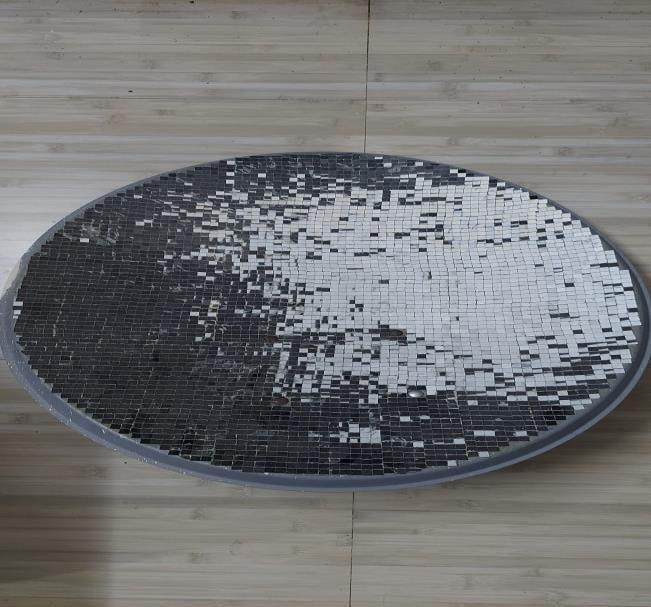
\includegraphics[width=68mm]{figures/fig1_parabolic_dish.jpg}
\end{center}

\vspace{2mm}
\noindent
\begin{spacing}{1.15}
{\fontsize{9.8}{13.5}\selectfont
The image shows the fabricated parabolic solar concentrator developed for this project, which is designed to focus sunlight onto a single focal point for efficient heat generation. The concentrator surface is constructed using multiple small square mirror pieces carefully arranged on a curved parabolic base to achieve the desired reflective geometry. Each mirror segment reflects incoming solar radiation toward the focal point, where a receiver tube or container is placed to absorb concentrated heat energy. This design allows the system to attain high temperatures suitable for water heating and steam generation, utilizing clean and renewable solar energy.\\[2.5mm]
The use of mirror tiles instead of a single reflective sheet significantly reduces fabrication costs while maintaining high reflectivity and durability. The circular structure provides better light focusing and structural stability. The concentrator, with a 60~cm diameter and 40~cm focal length, is integrated with a real-time automated solar tracking system to maintain optimal alignment with the sun throughout the day. This practical and cost-effective design demonstrates the potential of locally fabricated solar concentrators for sustainable thermal energy applications in domestic and industrial sectors. A parabolic concentrator is a reflective device that focuses incoming solar radiation onto a focal point or line. The design is based on the geometric properties of a parabola, where all rays parallel to the principal axis are reflected through a single focal point. In this project, a cylindrical parabolic concentrator is used to concentrate sunlight onto a receiver tube located at the focal point to achieve efficient heating and steam generation.
}
\end{spacing}
\clearpage


% --- Page 16 ---
% ==============================================================================
% PAGE 16: DESIGN PARAMETERS (Numbered Page 8)
% ==============================================================================
\begin{center}
  {\fontsize{14}{17}\selectfont \bfseries \underline{DESIGN PARAMETERS}}\\[4mm]
  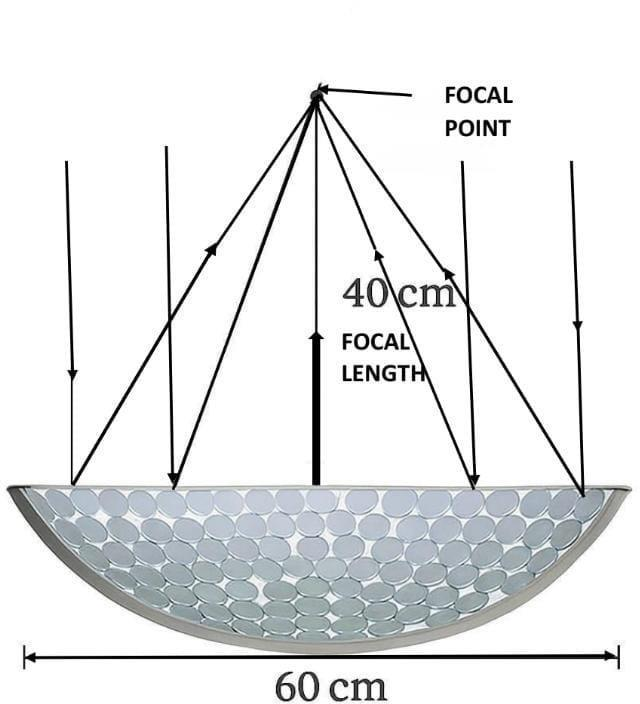
\includegraphics[width=85mm]{figures/fig_design_parameters.jpg}\\[6mm]
\end{center}

\noindent
{\fontsize{11}{16}\selectfont
\textbf{From the given design:}\\[4mm]
\textbf{Aperture Diameter (D):} 60 cm\\[3mm]
\textbf{Focal Length (f):} 40 cm\\[3mm]
\textbf{Shape:} Cylindrical Parabolic Reflector\\[3mm]
\textbf{Type:} Linear-focus concentrator\\[3mm]
\textbf{Material:} mirror-finished sheet\\[3mm]
\textbf{Receiver Position:} Placed along the focal line at a height equal to the focal length (40 cm from the vertex)
}
\clearpage


% --- Page 17 ---
% ==============================================================================
% PAGE 17: 2) RECEIVER (Numbered Page 9)
% ==============================================================================
\subsubsection*{2) RECEIVER}

\begin{center}
  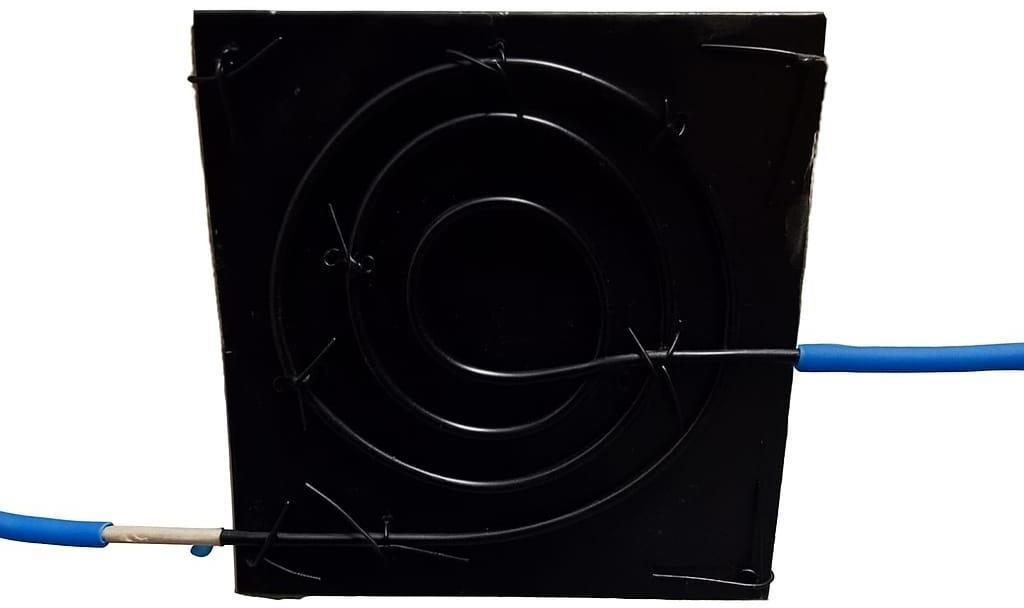
\includegraphics[width=90mm]{figures/fig2_receiver.jpg}
\end{center}

\vspace{3mm}
\noindent
\begin{spacing}{1.2}
{\fontsize{10.2}{14.5}\selectfont
In this project, the receiver plays a vital role in absorbing concentrated solar radiation and converting it into thermal energy. The receiver is fabricated from a copper coil with an internal diameter of 3~mm, selected for its excellent thermal conductivity and corrosion resistance. Copper is an ideal material for solar thermal systems as it ensures rapid heat transfer from the concentrated sunlight to the working fluid circulating inside the coil.\\[3mm]
The receiver coil is positioned precisely at the focal point of the parabolic concentrator, where maximum solar energy is focused.\\[3mm]
To enhance heat absorption and minimize reflective losses, the copper coil is coated with matte black heat-resistant paint. The black surface increases the absorptivity of the receiver, allowing it to capture a greater portion of incident solar radiation. The small internal diameter ensures a higher rate of heat transfer to the flowing water, enabling quick temperature rise and even steam generation under continuous solar exposure. This receiver design ensures efficient energy utilization and contributes significantly to the overall performance and thermal efficiency of the solar water heater and steam generator system.
}
\end{spacing}
\clearpage


% --- Page 18 ---
% ==============================================================================
% PAGE 18: 3) COLD WATER STORAGE TANK (Pre-Heating Unit) (Numbered Page 10)
% ==============================================================================
\subsubsection*{3) COLD WATER STORAGE TANK (Pre-Heating Unit)}

\begin{center}
  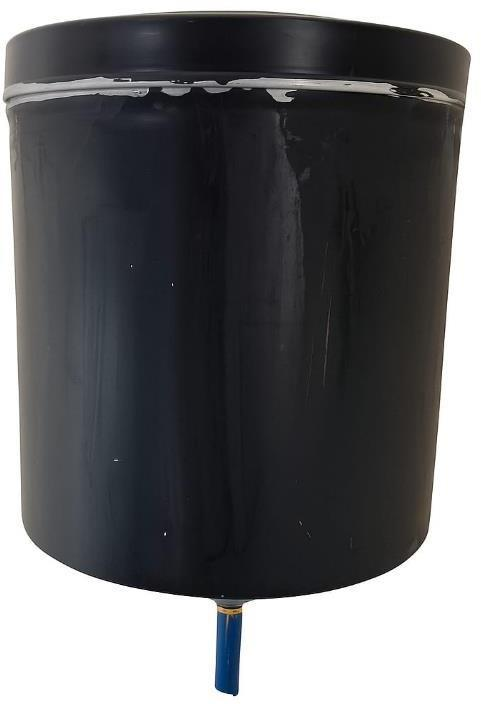
\includegraphics[width=50mm]{figures/fig3_cold_water_storage_tank.jpg}
\end{center}

\noindent
\begin{spacing}{1.2}
{\fontsize{10.2}{14.5}\selectfont
A black-colored cold storage water tank is installed as a pre-heating unit in the system. It serves two purposes:\\[3mm]
\textbf{SPECIFICATION:}
\begin{enumerate}[leftmargin=8mm, itemsep=2mm]
  \item \textbf{Pre-heating of water:} The black surface absorbs solar radiation effectively, slightly increasing the temperature of the water before it enters the copper receiver. This pre-heating process improves overall system efficiency and reduces the time required to reach the desired hot-water temperature.
  \item \textbf{Storage:} The tank also acts as a temporary storage reservoir that supplies a steady flow of water to the parabolic collector.\\[1.5mm]
  The tank is made of lightweight aluminium material, coated with black paint to maximize solar absorption.\\[1.5mm]
  A small outlet at the bottom connects to the copper receiver tube through a flexible pipe. This simple addition improves energy utilization and makes the design cost-effective and efficient.
  \item \textbf{Capacity of the tank :} 5 lit
\end{enumerate}
}
\end{spacing}
\clearpage


% --- Page 19 ---
% ==============================================================================
% PAGE 19: 4) WATER SUPPLY PIPE (Connecting Line) (Numbered Page 11)
% ==============================================================================
\subsubsection*{4) WATER SUPPLY PIPE (Connecting Line)}

\begin{center}
  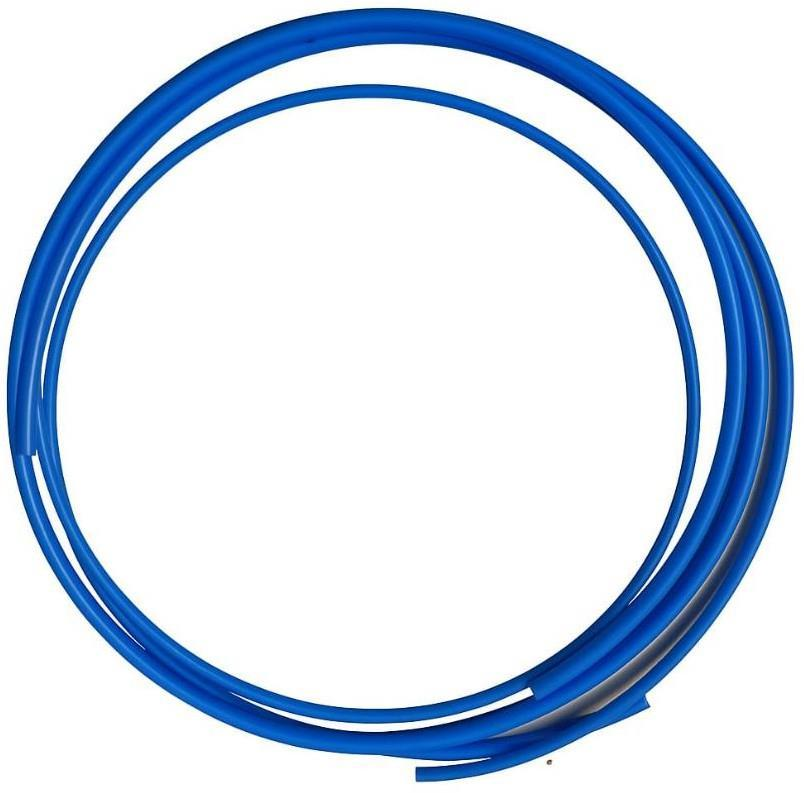
\includegraphics[width=65mm]{figures/fig4_water_supply_pipe.jpg}
\end{center}

\noindent
\begin{spacing}{1.2}
{\fontsize{10.2}{14.5}\selectfont
A flexible blue plastic pipe is used in the system to connect the cold storage water tank with the copper receiver tube. This pipe serves as the main water supply line and ensures a smooth, continuous flow of water from the tank to the receiver during operation.\\[3mm]
\textbf{Material and Function:}
\begin{itemize}[leftmargin=8mm, itemsep=1.5mm, label=\textbullet]
  \item The pipe is made of high-density polyethylene (HDPE), which is lightweight, durable, and resistant to heat and corrosion.
  \item It is capable of withstanding moderate pressure and temperature, making it suitable for small scale solar heating systems.
  \item The inner surface is smooth, allowing easy water flow with minimal frictional losses.
  \item Its blue color helps in identifying it as the cold-water line, preventing confusion with the hot-water outlet.
\end{itemize}
\vspace{2mm}
\textbf{Role in the Project:}
\begin{itemize}[leftmargin=8mm, itemsep=1.5mm, label=\textbullet]
  \item Carries water from the pre-heating storage tank to the copper receiver.
  \item Maintains a constant water level and flow rate in the heating section.
  \item Improves system performance by ensuring that no air pockets or leaks occur.
  \item Flexible enough to accommodate small movements in the solar tracking assembly.
\end{itemize}
}
\end{spacing}
\clearpage


% --- Page 20 ---
% ==============================================================================
% PAGE 20: 5) FLOW CONTROL VALVE (Hoffman Clamp Arrangement) (Numbered Page 12)
% ==============================================================================
\subsubsection*{5) FLOW CONTROL VALVE (Hoffman Clamp Arrangement)}

\begin{center}
  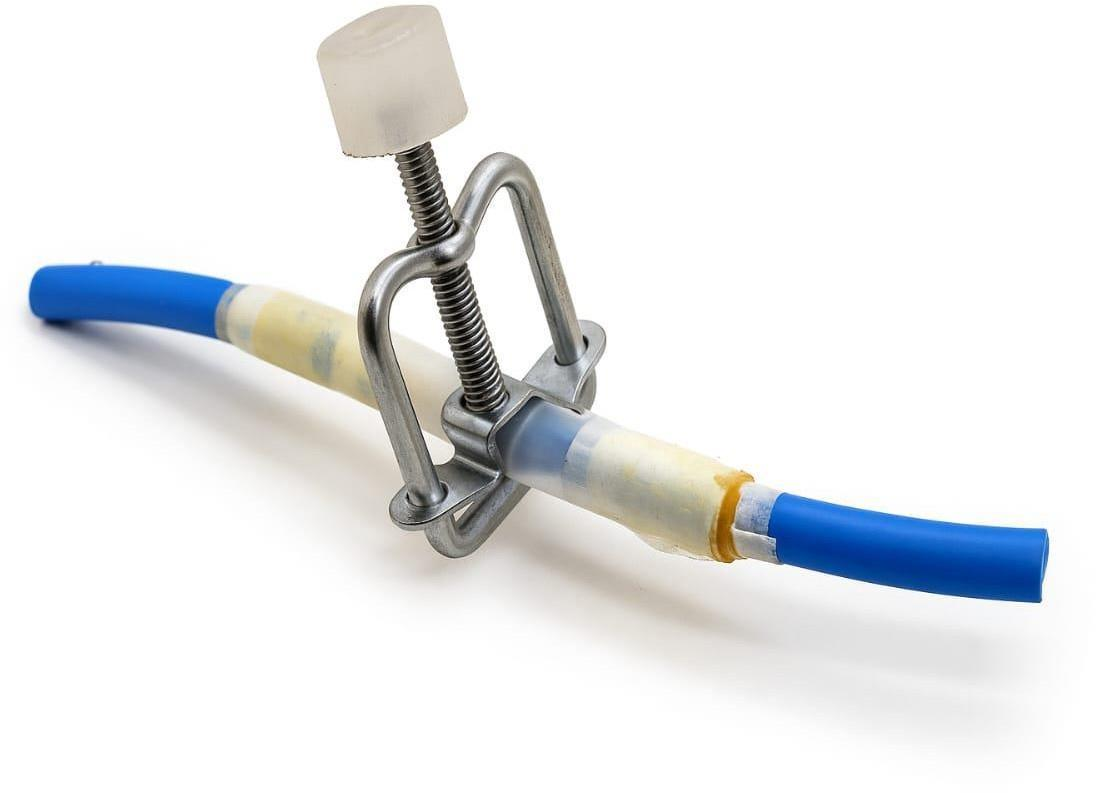
\includegraphics[width=80mm]{figures/fig5_flow_control_valve.jpg}
\end{center}

\noindent
\begin{spacing}{1.2}
{\fontsize{10.2}{14.5}\selectfont
A Hoffman clamp is used in the project as a manual flow control valve for the water passing through the blue supply pipe. It allows precise regulation of the water flow from the storage tank to the copper receiver tube, ensuring that the heating process remains efficient and steady.\\[3mm]
\textbf{Construction:}
\begin{itemize}[leftmargin=8mm, itemsep=1.5mm, label=\textbullet]
  \item The clamp consists of a U-shaped metal frame with a threaded screw and a knob at the top.
  \item The blue flexible pipe passes through the clamp opening.
  \item By rotating the knob clockwise, the screw presses against the pipe, restricting or stopping the water flow.
  \item Turning it anti-clockwise loosens the pressure, allowing smooth water passage.
\end{itemize}
\vspace{2mm}
\textbf{Function in the Project:}
\begin{enumerate}[leftmargin=8mm, itemsep=2mm]
  \item Controls the rate of water flow to maintain proper heat absorption in the copper tube.
  \item Prevents wastage of hot water and maintains uniform temperature rise.
  \item Acts as a simple and low-cost valve system, eliminating the need for expensive plumbing fittings.
  \item Makes the experimental setup easy to adjust during testing. This component ensures better temperature control and improves the overall performance and efficiency of the solar water heater.
\end{enumerate}
}
\end{spacing}
\clearpage


% --- Page 21 ---
% ==============================================================================
% PAGE 21: 6) ARDUINO NANO (Numbered Page 13)
% ==============================================================================
\subsubsection*{6) ARDUINO NANO}

\begin{center}
  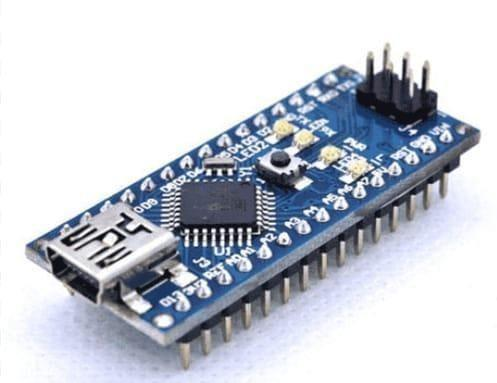
\includegraphics[width=65mm]{figures/fig6_arduino_nano.jpg}
\end{center}

\noindent
\begin{spacing}{1.2}
{\fontsize{10.2}{14.5}\selectfont
The Arduino Nano is a compact, microcontroller-based development board used as the main control unit in the solar tracking system of this project. It is responsible for processing the signals received from the Light Dependent Resistors (LDRs) and controlling the PMDC motor through the motor driver module, ensuring that the parabolic collector continuously follows the Sun's position throughout the day.\\[3.5mm]
\textbf{Function:}
\begin{itemize}[leftmargin=8mm, itemsep=2mm, label=\textbullet]
  \item Two LDR sensors are mounted on opposite sides of the collector.
  \item When sunlight intensity Differs between the two sensors, the Arduino Nano detects the voltage difference.
  \item It sends a control signal to the motor driver circuit, which activates the PMDC motor to rotate the collector toward the brighter side (toward the Sun).
  \item Once both LDRs sense equal light, the Arduino stops the motor --- meaning the collector is correctly aligned with the Sun.
\end{itemize}
}
\end{spacing}
\clearpage


% --- Page 22 ---
% ==============================================================================
% PAGE 22: 7) MOTOR DRIVER UNIT (Numbered Page 14)
% ==============================================================================
\subsubsection*{7) MOTOR DRIVER UNIT}

\begin{center}
  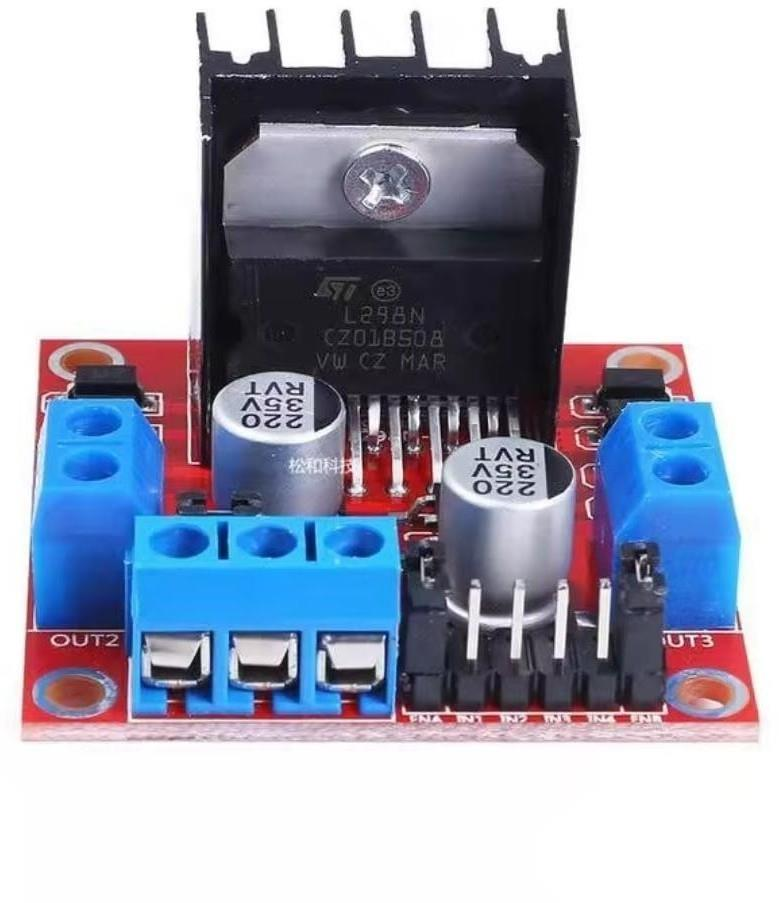
\includegraphics[width=55mm]{figures/fig7_motor_driver.jpg}
\end{center}

\noindent
\begin{spacing}{1.2}
{\fontsize{10.2}{14.5}\selectfont
The motor driver unit used in my project is an L298N motor driver module, which is designed to control the speed and direction of a Permanent Magnet DC (PMDC) motor. It acts as an interface between the microcontroller and the motor because a microcontroller cannot supply the high current required by the motor. The L298N is a dual H-bridge motor driver IC that can control two PMDC motors or one stepper motor. It operates using an external power supply (usually 5V--35V) and provides sufficient current (up to 2A per channel) to drive the motors efficiently.\\[3.5mm]
\textbf{Function:}
\begin{itemize}[leftmargin=8mm, itemsep=2mm, label=\textbullet]
  \item The motor driver works on the H-bridge principle, which allows the motor to rotate in both forward and reverse directions.
  \item When control signals from the microcontroller are applied to the input pins, the driver sends the proper polarity of voltage to the motor terminals.
  \item By changing the logic of the inputs, the direction of current through the motor changes, which changes the rotation direction.
  \item The enable pins control the motor speed using Pulse Width Modulation (PWM) signals.
  \item Thus, the L298N motor driver helps to easily control the speed and direction of a PMDC motor in the project.
\end{itemize}
}
\end{spacing}
\clearpage


% --- Page 23 ---
% ==============================================================================
% PAGE 23: 8) LDR SENSOR MODULE (Numbered Page 15)
% ==============================================================================
\subsubsection*{8) LDR SENSOR MODULE (Light Detection Unit)}

\begin{center}
  \begin{tabular}{cc}
    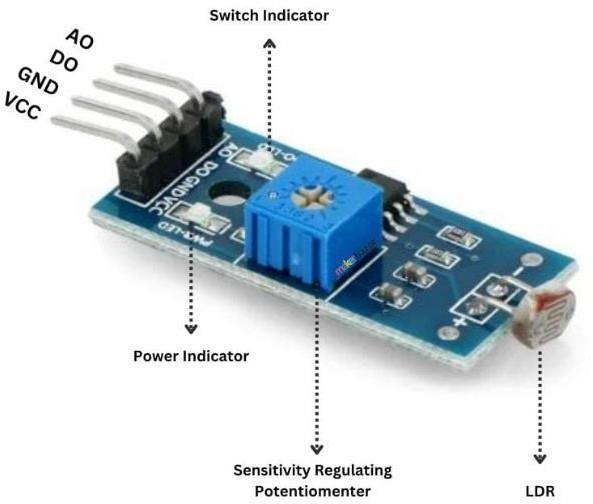
\includegraphics[width=48mm]{figures/fig8_ldr_sensor_module.jpg} &
    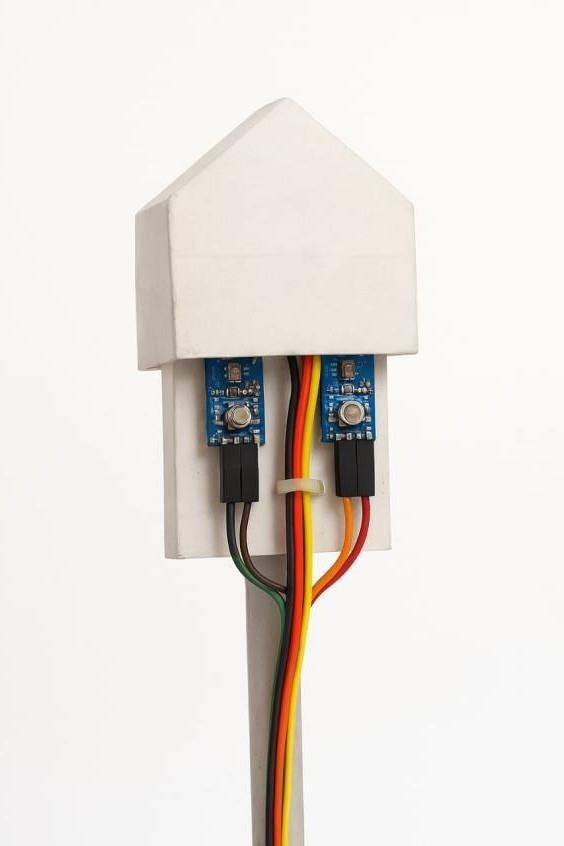
\includegraphics[width=42mm]{figures/fig8b_ldr_dual_module.jpg}
  \end{tabular}
\end{center}

\noindent
\begin{spacing}{1.2}
{\fontsize{10.2}{14.5}\selectfont
The LDR (Light Dependent Resistor) sensor module is used in this project to detect the intensity of sunlight and provide input to the Arduino Nano for automatic solar tracking. It works on the principle that the resistance of an LDR changes with the intensity of light falling on it.\\[3.5mm]
\textbf{Function:}
\begin{itemize}[leftmargin=8mm, itemsep=2mm, label=\textbullet]
  \item Two LDR modules are placed at slightly different positions on the parabolic collector.
  \item When sunlight intensity is unequal between the two sensors, the resistance difference creates a voltage difference.
  \item This voltage difference is sent to the Arduino Nano, which processes the signal.
  \item The Arduino then commands the motor driver to rotate the collector toward the side receiving less light, aligning it perfectly with the Sun.
  \item Once both LDRs sense equal sunlight, the system stops the motor --- indicating correct alignment.
\end{itemize}
}
\end{spacing}
\clearpage


% --- Page 24 ---
% ==============================================================================
% PAGE 24: 9) PUSH BUTTONS (Numbered Page 16)
% ==============================================================================
\subsubsection*{9) PUSH BUTTONS}

\begin{center}
  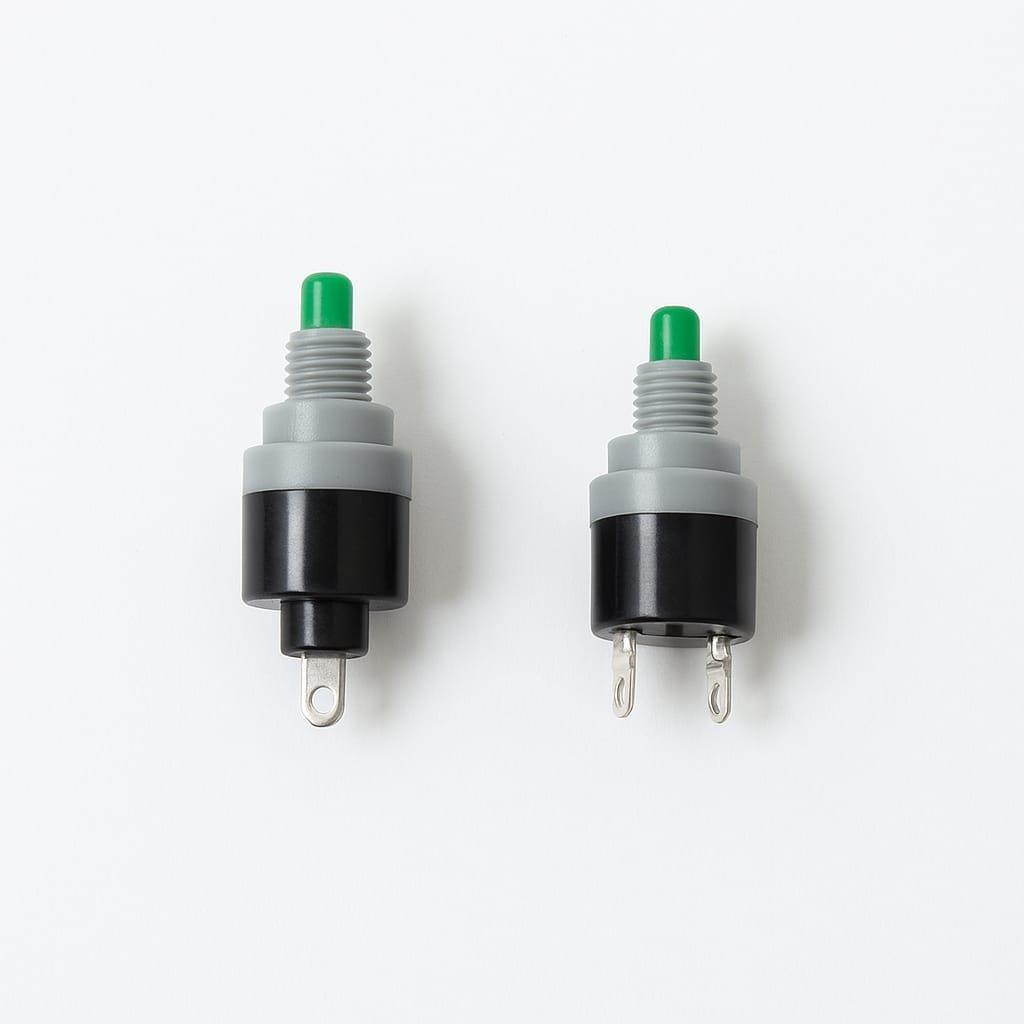
\includegraphics[width=65mm]{figures/fig9_push_buttons.jpg}
\end{center}

\noindent
\begin{spacing}{1.2}
{\fontsize{10.2}{14.5}\selectfont
Push button switches are used as control inputs to operate the motor's direction of rotation. These push buttons are simple, momentary-type switches that make or break an electrical connection when pressed. They are compact, easy to use, and reliable for controlling electronic circuits. Each button is connected to the control pins of the motor driver circuit, which in turn determines the motor's movement direction.\\[3.5mm]
\textbf{Function:}
\begin{itemize}[leftmargin=8mm, itemsep=2mm, label=\textbullet]
  \item There are two push buttons used in the project --- one for right (forward) rotation and the other for left (reverse) rotation of the PMDC motor.
  \item When the right push button is pressed, it sends a signal to the motor driver to rotate the motor in the forward direction.
  \item Similarly, pressing the left push button changes the signal polarity through the driver, causing the motor to rotate in the reverse direction.
  \item Once the button is released, the circuit opens, and the motor stops.
  \item This simple push button control allows easy and manual direction control of the motor.
\end{itemize}
}
\end{spacing}
\clearpage


% --- Page 25 ---
% ==============================================================================
% PAGE 25: 9) PERMANENT MAGNET DIRECT CURRENT (PDMC) MOTOR (Numbered Page 17)
% ==============================================================================
\subsubsection*{9) PERMANENT MAGNET DIRECT CURRENT (PDMC) MOTOR}

\begin{center}
  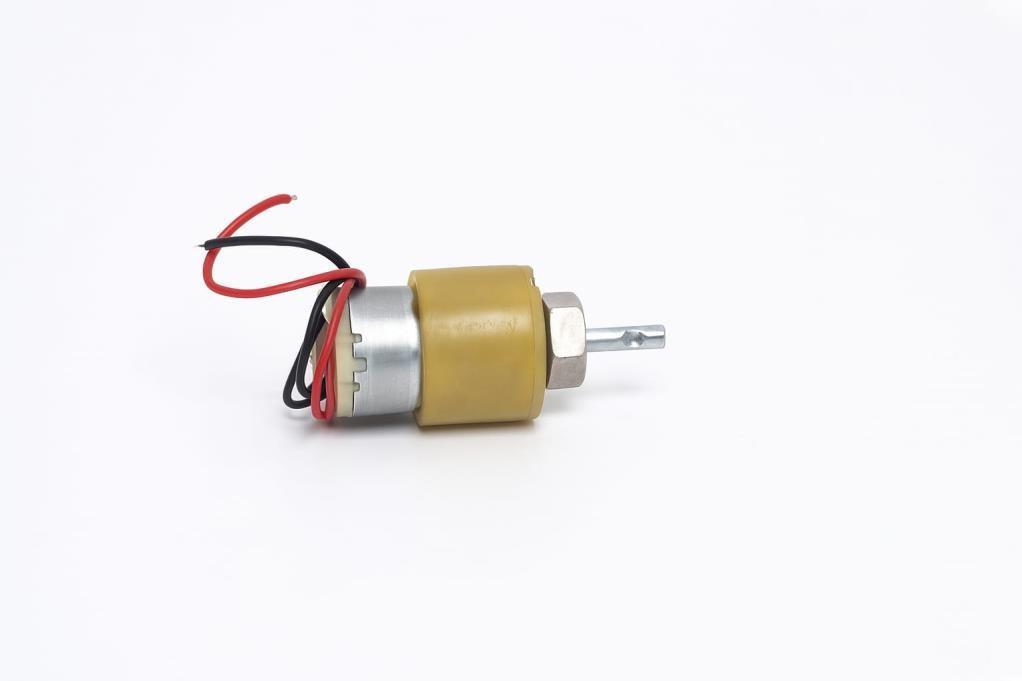
\includegraphics[width=70mm]{figures/fig10_pmdc_motor.jpg}
\end{center}

\noindent
{\fontsize{10.5}{15}\selectfont
\textbf{Specifications}\\[1.5mm]
\textbf{Voltage:} 6V or 9V DC\\[1.5mm]
\textbf{Speed:} 100--300 RPM (depends on load)\\[1.5mm]
\textbf{Power:} 5--15 Watts\\[1.5mm]
\textbf{Control:} Easily reversible by changing polarity\\[3.5mm]
\textbf{Function}\\[2mm]
\textbf{1. Tracking Motion:}\\
The motor is used to rotate the dish (either horizontally or vertically) to follow the sun's movement throughout the day. It ensures maximum solar radiation is focused on the receiver.\\[2.5mm]
\textbf{2. Automatic Control:}\\
The motor operates through a motor driver and sensor system (like LDR sensors) that detect sunlight direction.\\[2.5mm]
\textbf{3. Power Source:}\\
It is powered by a battery or solar panel output, making the system self-sustainable.
}
\clearpage


% --- Page 26 ---
% ==============================================================================
% PAGE 26: 10) V-GROOVE BELT AND PULLY (Numbered Page 18)
% ==============================================================================
\subsubsection*{10) V-GROOVE BELT AND PULLY}

\begin{center}
  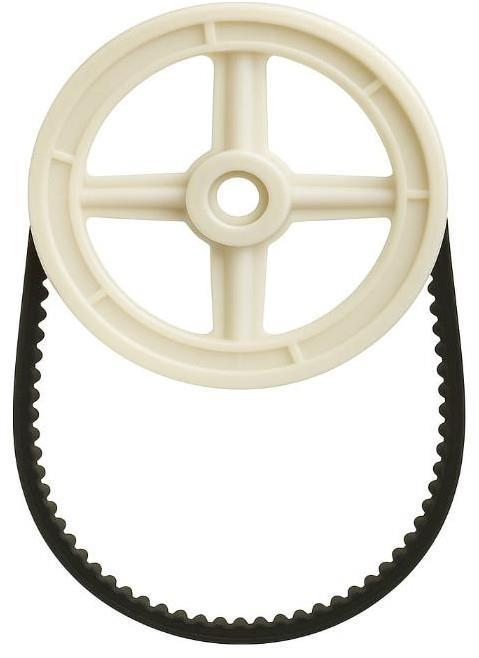
\includegraphics[width=48mm]{figures/fig11_v_groove_belt_pulley.jpg}
\end{center}

\noindent
\begin{spacing}{1.2}
{\fontsize{10.2}{14.5}\selectfont
\textbf{Specifications of V-Groove Belt and Pulley}
\begin{enumerate}[leftmargin=8mm, itemsep=2mm]
  \item Type of drive -- V-belt drive
  \item Belt type -- V-groove
  \item Belt material -- Reinforced rubber
  \item Belt length -- Around 600 mm to 800 mm
  \item Driven pulley diameter -- 25 cm (250 mm)
  \item Driver pulley diameter -- 5 cm to 10 cm (mounted on motor shaft)
  \item Speed ratio -- 1 : 2.5 to 1 : 5 (for speed reduction and torque increase)
  \item Driver pulley material -- Mild steel or aluminum alloy
  \item Driven pulley material -- Fiber
  \item Center distance between shafts -- 175 mm to 180 mm (adjustable)
\end{enumerate}
}
\end{spacing}
\clearpage


% --- Page 27 ---
% ==============================================================================
% PAGE 27: FUNCTION OF BELT AND PULLEY (Numbered Page 19)
% ==============================================================================
\subsubsection*{Function}
\vspace{3mm}

\noindent
\begin{spacing}{1.3}
{\fontsize{10.5}{15.5}\selectfont
\textbf{1. Power Transmission:}\\
The V-groove belt connects the PMDC motor to the dish rotation shaft via the 25 cm pulley. It transmits the rotational motion from the motor to the parabolic dish assembly.\\[4mm]
\textbf{2. Speed Reduction and Torque Increase:}\\
A larger pulley (25 cm) helps reduce speed and increase torque, which is ideal for slow and steady dish rotation.\\[4mm]
\textbf{3. Smooth and Silent Operation:}\\
The V-belt drive provides smooth, shock-free motion with minimal vibration and noise.\\[4mm]
\textbf{4. Protection Against Overload:}\\
If the dish is obstructed, the belt may slip slightly, protecting the motor from damage.\\[4mm]
\textbf{5. Easy Maintenance:}\\
Simple to install, adjust, and replace; no lubrication required.
}
\end{spacing}
\clearpage


% --- Page 28 ---
% ==============================================================================
% PAGE 28: 10) BATTERY(6V,6AMP) (Numbered Page 20)
% ==============================================================================
\subsubsection*{10) BATERY(6V,6AMP)}

\begin{center}
  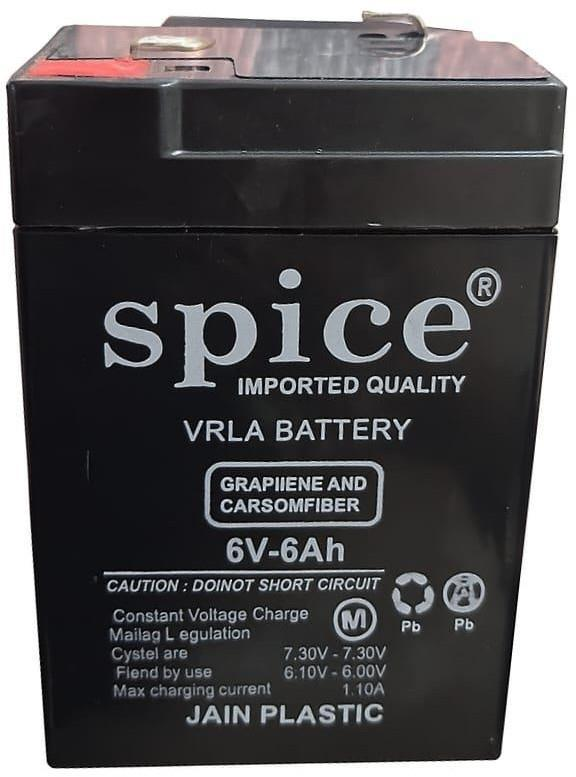
\includegraphics[width=55mm]{figures/fig12_battery.jpg}
\end{center}

\noindent
\begin{spacing}{1.2}
{\fontsize{10.2}{14.5}\selectfont
The system uses a Spice VRLA Battery (6V, 6Ah) made with graphene and carbon fiber technology. It is a sealed lead-acid, maintenance-free battery that provides stable DC power for operating the motor and sensors.\\[3mm]
\textbf{Main Specifications:}
\begin{itemize}[leftmargin=8mm, itemsep=1.5mm, label=\textbullet]
  \item \textbf{Type:} VRLA (Valve Regulated Lead Acid) Battery
  \item \textbf{Rated Voltage:} 6V
  \item \textbf{Capacity:} 6Ah
  \item \textbf{Charging Voltage:} 7.2V -- 7.5V (Cycle use)
  \item \textbf{Standby Voltage:} 6.78V -- 6.90V
  \item \textbf{Maximum Charging Current:} 1.35A
  \item \textbf{Features:} Maintenance-free, long service life, and safe sealed design
\end{itemize}
\vspace{2mm}
This battery ensures reliable power supply for small DC motors and electronic sensor circuits in the project.
}
\end{spacing}
\clearpage


% --- Page 29 ---
% ==============================================================================
% PAGE 29: 11) SOLAR PANEL UNIT (Numbered Page 21)
% ==============================================================================
\subsubsection*{11) SOLAR PANEL UNIT}

\begin{center}
  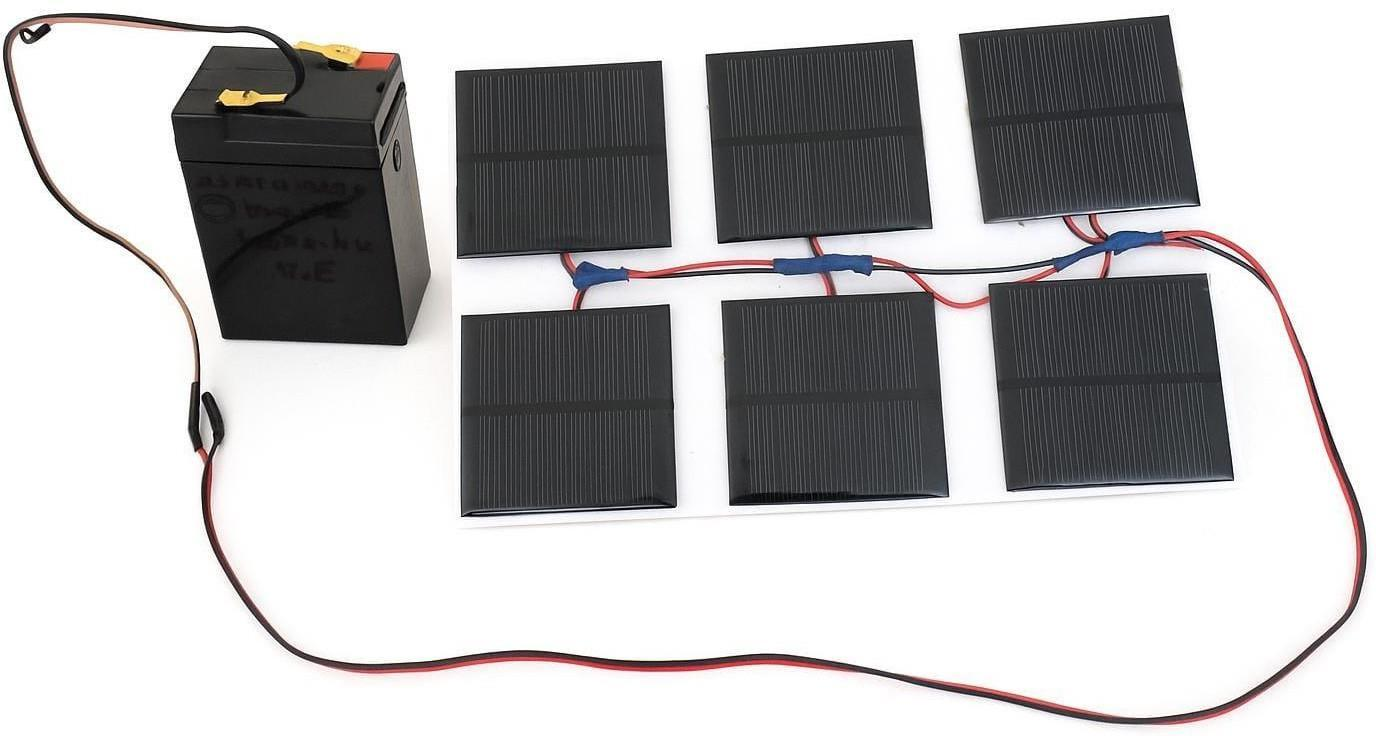
\includegraphics[width=90mm]{figures/fig13_solar_panel_unit.jpg}
\end{center}

\noindent
\begin{spacing}{1.2}
{\fontsize{10.2}{14.5}\selectfont
A solar panel unit is used as the main source of electrical power generation. Each solar panel is capable of producing around 6 amperes of current, and when connected together in a suitable configuration, the entire system generates a total output voltage of about 10 to 12 volts. This generated DC power is used for charging the battery, which later supplies energy to the control and motor units of the system. Solar energy is a renewable and eco-friendly source, making the setup efficient and sustainable for long-term operation.\\[3mm]
To ensure safe operation, a diode is connected in the circuit to allow one-way power flow from the solar panels to the battery. This prevents the reverse flow of current, protecting the solar panels from short-circuiting or back current during low or no sunlight conditions. This arrangement helps maintain the reliability and safety of the charging system.
}
\end{spacing}
\clearpage


% --- Page 30 ---
% ==============================================================================
% PAGE 30: 12) WOODEN BASE, PVC PIPE & VARIOUS TYPES OF NUT (Numbered Page 22)
% ==============================================================================
\subsubsection*{12) WOODEN BASE, PVC PIPE \& VARIOUS TYPES OF NUT}

\begin{center}
  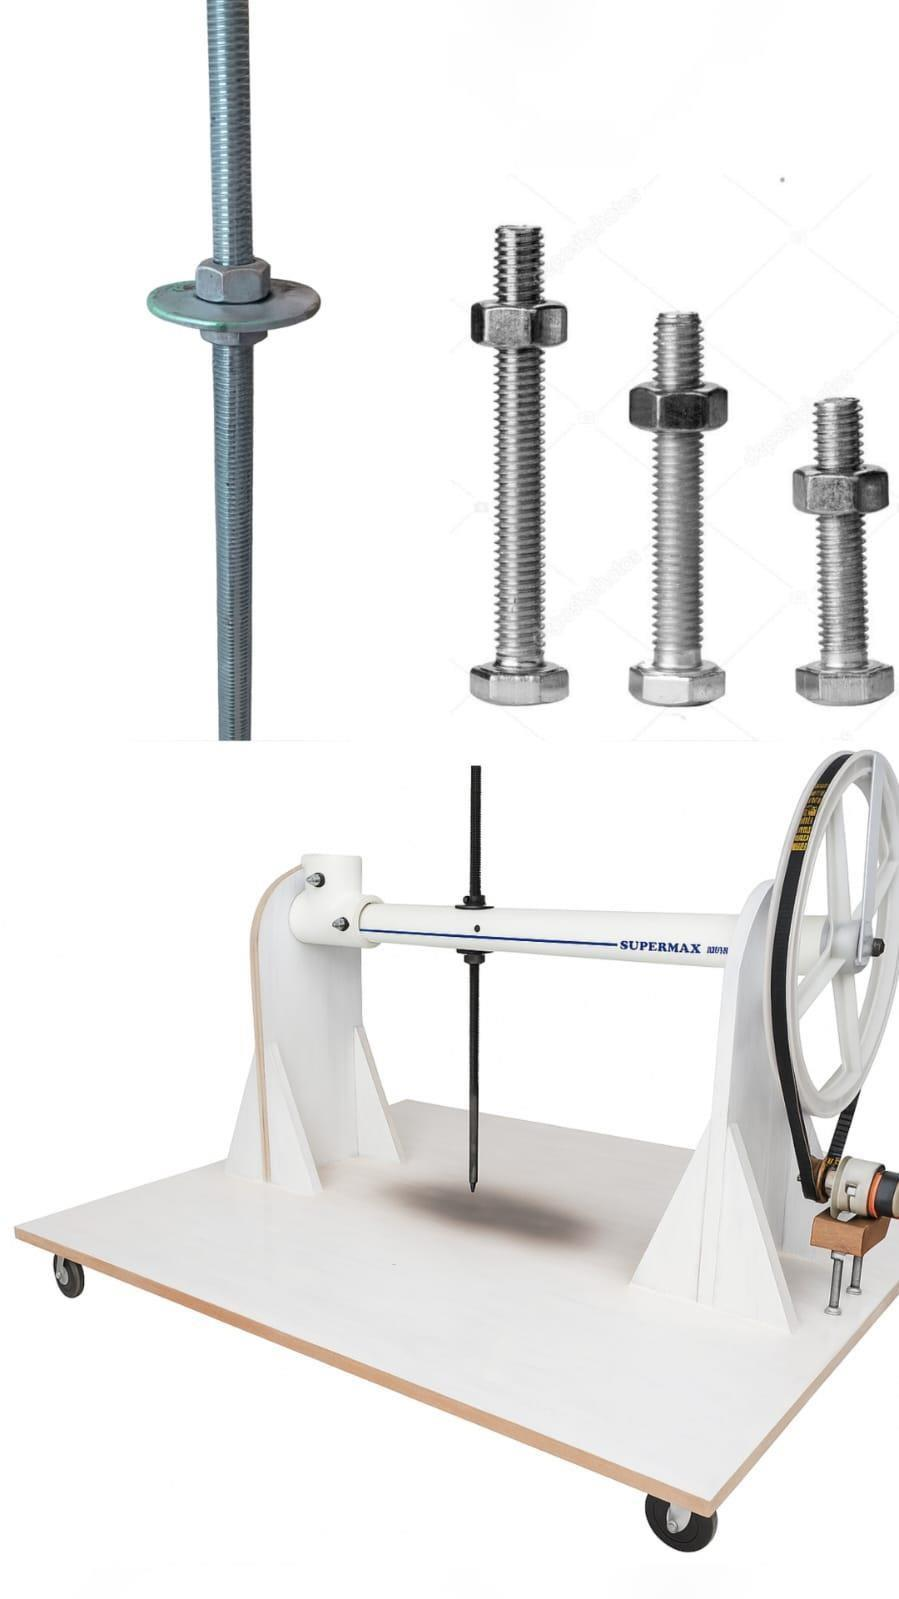
\includegraphics[width=75mm]{figures/fig14_wooden_base_assembly.jpg}
\end{center}

\noindent
\begin{spacing}{1.2}
{\fontsize{10.2}{14.5}\selectfont
The stud rod is a fully threaded rod that provides adjustable connections using nuts and washers at both ends. Different types of nuts and bolts are used to fix and support various parts of the assembly securely. The PVC pipe acts as the main shaft, on which the pulley is mounted. This shaft transmits rotational motion from the motor to the parabolic dish, allowing smooth and stable operation.\\[3mm]
The motor and pulley arrangement are connected through a belt drive, which transfers torque efficiently to the PVC shaft. The base platform of size 60 $\times$ 60 cm is made from a wooden sheet, providing a strong and stable foundation for the entire setup. This design ensures that all components remain firmly in place during the operation and allows precise and balanced rotation of the parabolic dish for tracking or positioning purposes.
}
\end{spacing}
\clearpage


% --- Page 31 ---
% ==============================================================================
% PAGE 31: 3.2 SOLAR TRACKING MECHANISM - INTRODUCTION (Numbered Page 23)
% ==============================================================================
\subsection*{3.2) SOLAR TRACKING MECHANISM :}

\begin{center}
  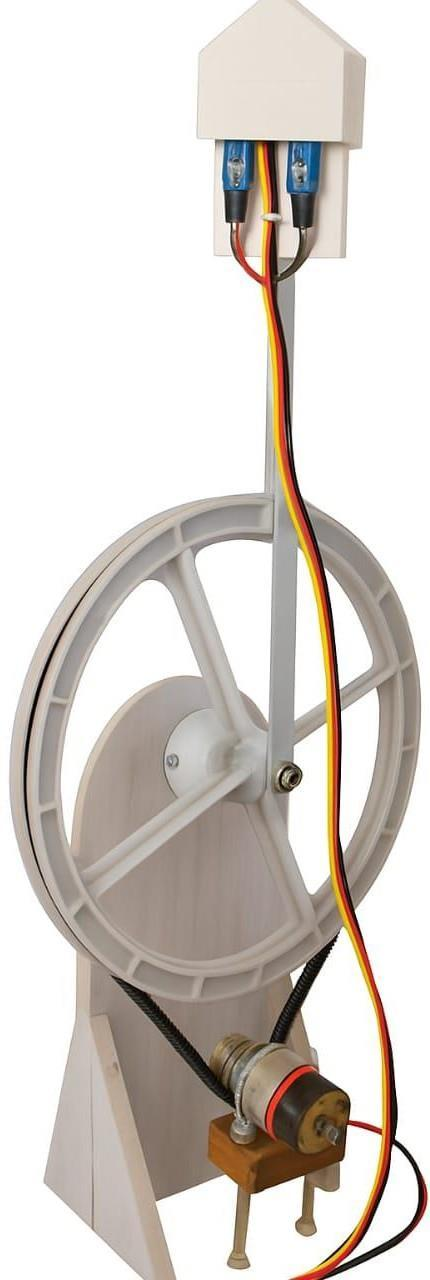
\includegraphics[width=45mm]{figures/fig15_solar_tracking_mechanism.jpg}
\end{center}

\subsubsection*{1. Introduction}
\noindent
\begin{spacing}{1.25}
{\fontsize{10.2}{15}\selectfont
The single-axis solar tracking mechanism is used to automatically rotate the parabolic dish from east to west to follow the sun's movement.\\[2.5mm]
It helps maintain maximum sunlight focus on the receiver throughout the day.\\[2.5mm]
The system works using LDR sensors, a PMDC motor, and a control circuit powered by solar energy.\\[2.5mm]
This automatic motion increases the overall efficiency and heat output of the solar water heater. It is a simple, low-cost, and effective method for improving solar energy utilization.
}
\end{spacing}
\clearpage


% --- Page 32 ---
% ==============================================================================
% PAGE 32: TRACKING COMPONENTS & WORKING PRINCIPLE (Numbered Page 24)
% ==============================================================================
\subsubsection*{2. Type of Tracking}
\noindent
{\fontsize{10}{14}\selectfont
\textbf{Type:} Single Axis Automatic Tracking\\[1mm]
\textbf{Axis of Rotation:} East--West (horizontal axis)\\[1mm]
\textbf{Purpose:} To maintain continuous alignment of the parabolic dish with the moving sun during the day.\\[1mm]
\textbf{Control:} Automatic using sensors and motor.
}

\vspace{3mm}
\subsubsection*{3. Components of Single Axis Tracking System}
\begin{center}
\renewcommand{\arraystretch}{1.2}
\begin{tabular}{|p{42mm}|p{82mm}|}
\hline
\rowcolor{gray!20}
\textbf{Component} & \textbf{Specification / Function} \\
\hline
LDR Sensors (2 No.) & Detect sunlight intensity difference on both sides \\
\hline
Control Circuit / Comparator & Compares LDR signals and controls motor direction \\
\hline
PMDC Motor (6--9V, 10--15W) & Provides rotary motion for dish movement \\
\hline
Motor Driver (L293D / Relay) & Drives motor forward or reverse based on sensor input \\
\hline
V-Groove Belt \& Pulley (25 cm Pulley) & Transfers motion from motor to dish \\
\hline
Power Supply & 12V DC battery charged by small solar panel \\
\hline
Dish Support Frame & Allows rotation of dish around single horizontal axis \\
\hline
\end{tabular}
\end{center}

\vspace{2mm}
\subsubsection*{4. Working Principle}
\noindent
{\fontsize{10}{14}\selectfont
\textbf{$\blacklozenge$ Sensing Sunlight:}
\begin{itemize}[leftmargin=6mm, itemsep=1mm, label=\textbullet]
  \item Two LDR sensors are placed on either side of a small divider.
  \item When sunlight falls equally on both $\rightarrow$ system is balanced $\rightarrow$ motor off.
\end{itemize}
\textbf{$\blacklozenge$ Sun Movement:}
\begin{itemize}[leftmargin=6mm, itemsep=1mm, label=\textbullet]
  \item As the sun shifts from East to West, one LDR receives more light.
  \item The control circuit detects the difference in voltage between LDRs.
\end{itemize}
}
\clearpage


% --- Page 33 ---
% ==============================================================================
% PAGE 33: TRACKING ACTIVATION & ADVANTAGES (Numbered Page 25)
% ==============================================================================
\noindent
{\fontsize{10.2}{14.5}\selectfont
\textbf{$\blacklozenge$ Motor Activation:}
\begin{itemize}[leftmargin=6mm, itemsep=1.5mm, label=\textbullet]
  \item The comparator or controller sends a signal to the motor driver.
  \item The PMDC motor rotates the dish toward the brighter side.
\end{itemize}

\vspace{2mm}
\textbf{$\blacklozenge$ Balancing:}
\begin{itemize}[leftmargin=6mm, itemsep=1.5mm, label=\textbullet]
  \item When both sensors receive equal light again, the motor stops.
  \item The dish stays aligned with the sun automatically.
\end{itemize}

\vspace{2mm}
\textbf{$\blacklozenge$ End of Day:}
\begin{itemize}[leftmargin=6mm, itemsep=1.5mm, label=\textbullet]
  \item The dish remains in the West position at sunset.
  \item It can be manually or automatically reset to the East in the morning.
\end{itemize}
}

\vspace{4mm}
\subsubsection*{5. Functions of Tracking Mechanism}
\begin{itemize}[leftmargin=8mm, itemsep=2mm, label=\textbullet]
  \item Continuously aligns the dish with the sun's position.
  \item Ensures maximum solar radiation is focused on the receiver.
  \item Eliminates need for manual adjustment.
  \item Increases water heating and overall system efficiency.
  \item Operates using solar power, making it self-sufficient.
\end{itemize}

\vspace{4mm}
\subsubsection*{6. Advantages}
\begin{itemize}[leftmargin=8mm, itemsep=2mm, label=\textbullet]
  \item Simple and cost-effective compared to dual-axis systems.
  \item Reduces human effort.
  \item Compact and energy-efficient.
  \item Ideal for small- to medium-size parabolic dish systems.
  \item Improves output by 20--30\% over fixed-position setup.
\end{itemize}
\clearpage


% --- Page 34 ---
% ==============================================================================
% PAGE 34: CHAPTER-4 FABRICATION - PART 1 (Numbered Page 26)
% ==============================================================================
\begin{center}
  {\fontsize{15}{18}\selectfont \bfseries \textcolor{red!80!black}{\underline{CHAPTER-4}}}\\[2mm]
  {\fontsize{16}{20}\selectfont \bfseries \textcolor{red!80!black}{\underline{FABRICATION}}}\\[5mm]
\end{center}

\subsubsection*{1. Frame Construction}
\noindent
\begin{spacing}{1.2}
{\fontsize{10.2}{14.5}\selectfont
The base frame is made of wooden sheet ($60 \times 60$~cm) to provide stability and support to the setup. Holes are drilled to fix the shaft supports at the center.\\[2.5mm]
The frame is painted by white colour because it reflect solar rays to prevent electronic component from over heating.
}
\end{spacing}

\vspace{4mm}
\subsubsection*{2. Parabolic Dish Fabrication}
\noindent
\begin{spacing}{1.2}
{\fontsize{10.2}{14.5}\selectfont
A parabolic dish is made using satellite dish for lightweight and good reflection.\\[2.5mm]
The dish surface is covered with reflective mirror pieces to concentrate sunlight at the focus point. The dish is mounted on a PVC pipe shaft that allows rotational motion.
}
\end{spacing}

\vspace{4mm}
\subsubsection*{3. Receiver Fabrication}
\noindent
\begin{spacing}{1.2}
{\fontsize{10.2}{14.5}\selectfont
The receiver pipe (usually copper tube) is placed at the focal point of the parabola dish.\\[2.5mm]
The copper tube is black-painted for maximum heat absorption. The tube is connected with inlet and outlet pipes to circulate water.\\[2.5mm]
Copper tube is placed on the insulating material (aluminium plate and glass wool) for reducing heat loss.
}
\end{spacing}

\vspace{4mm}
\subsubsection*{4. Tracking Mechanism}
\noindent
\begin{spacing}{1.2}
{\fontsize{10.2}{14.5}\selectfont
A single-axis solar tracking system is used to follow the sun's motion east to west.\\[2.5mm]
A PMDC motor with pulley and V-belt attached with the PVC pipe shaft which is used to rotate the parabolic dish. Sensors (LDRs) are placed on both sides of the dish to detect sunlight intensity difference.\\[2.5mm]
A motor driver circuit and microcontroller (Arduino nano) control the motor rotation based on sensor signals.
}
\end{spacing}
\clearpage


% --- Page 35 ---
% ==============================================================================
% PAGE 35: FABRICATION - PART 2 (Numbered Page 27)
% ==============================================================================
\subsubsection*{5. Power Supplying Unit (Solar Panel \& Battery)}
\noindent
\begin{spacing}{1.2}
{\fontsize{10.2}{14.5}\selectfont
A small solar panel (12V) is mounted on the base frame or beside the dish.\\[2.5mm]
The panel converts sunlight into electrical energy to charge a 6V battery.\\[2.5mm]
The battery supplies power to the motor driver, sensors, and control circuit for automatic tracking.\\[2.5mm]
A blocking diode is used to ensure one-way current flow from the panel to the battery, preventing discharge at night.
}
\end{spacing}

\vspace{4mm}
\subsubsection*{6. Water Circulation System}
\noindent
\begin{spacing}{1.2}
{\fontsize{10.2}{14.5}\selectfont
Water from the storage tank which is placed at a certain height for direct flow of water to the inlet of receiver tube.\\[2.5mm]
Heated water exits from the outlet of the receiver tube and is collected in another container.
}
\end{spacing}

\vspace{4mm}
\subsubsection*{7. Assembly \& Testing}
\noindent
\begin{spacing}{1.2}
{\fontsize{10.2}{14.5}\selectfont
All components (frame, dish, receiver, motor, sensors, battery) are assembled.\\[2.5mm]
The system is tested under sunlight to check tracking accuracy and water temperature rise. Temperature readings are taken at regular intervals for performance analysis.
}
\end{spacing}

\vspace{4mm}
\subsubsection*{8. Finishing}
\noindent
\begin{spacing}{1.2}
{\fontsize{10.2}{14.5}\selectfont
Wiring is neatly arranged using cable ties.\\[2.5mm]
Components are painted or coated to prevent corrosion.\\[2.5mm]
Labels are added for inlet, outlet, and electrical parts for clarity.
}
\end{spacing}
\clearpage


% --- Page 36 ---
% ==============================================================================
% PAGE 36: CHAPTER-5 CONSTRUCTION - PART 1 (Numbered Page 28)
% ==============================================================================
\begin{center}
  {\fontsize{15}{18}\selectfont \bfseries \textcolor{red!80!black}{\underline{CHAPTER-5}}}\\[2mm]
  {\fontsize{16}{20}\selectfont \bfseries \textcolor{red!80!black}{\underline{CONSTRUCTION}}}\\[4mm]
  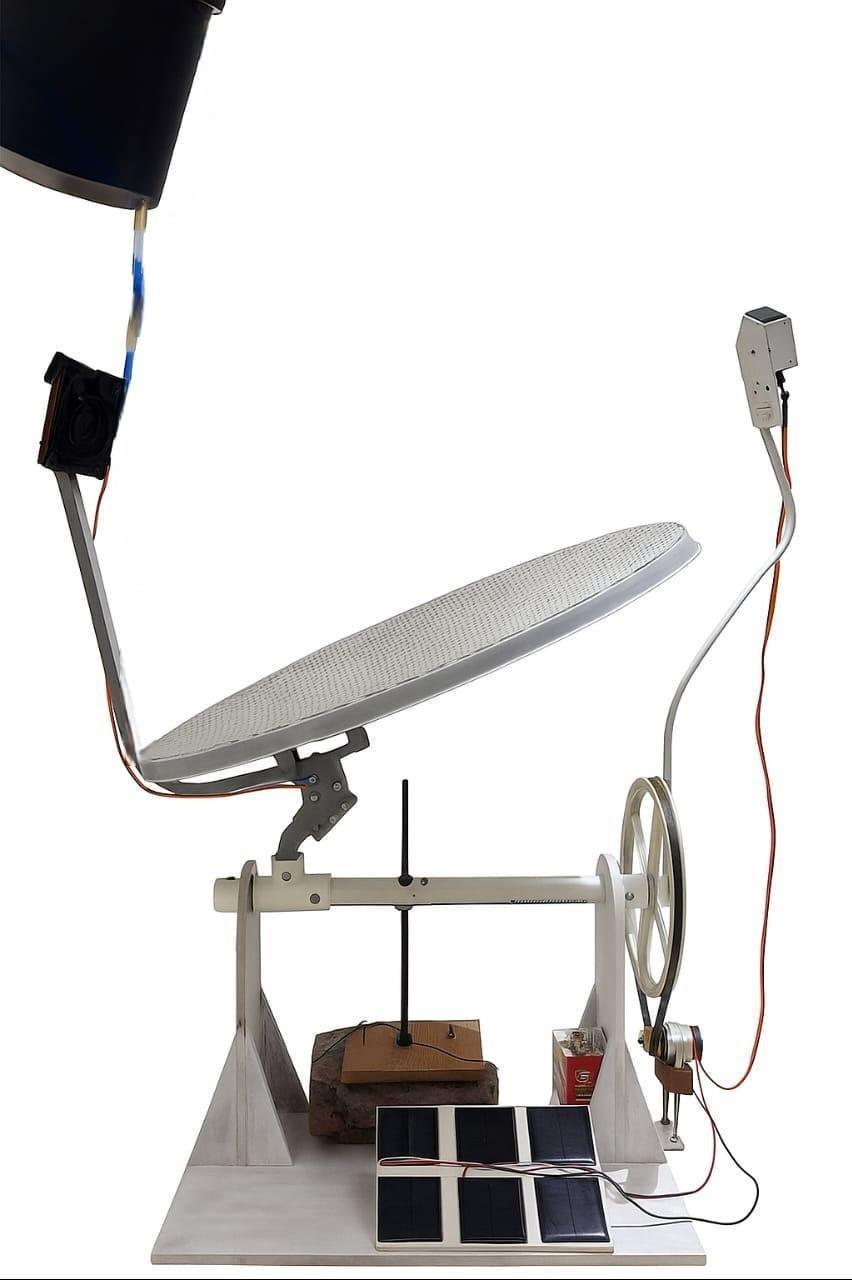
\includegraphics[width=90mm]{figures/fig16_actual_model.jpg}\\[5mm]
\end{center}

\noindent
\begin{spacing}{1.2}
{\fontsize{10.2}{14.5}\selectfont
The construction of the Parabolic Solar Water Heater with Automatic Tracking and Power Generation begins with preparing a strong base structure. A wooden sheet of $60\text{ cm} \times 60\text{ cm}$ is used as the base platform to support all components. A PVC pipe shaft is mounted horizontally at the center of this base to act as the main support for the parabolic dish. The end caps are fitted at the end of the shaft to allow smooth rotational movement. The base and supporting parts are properly aligned, drilled, and painted with white colour to prevent damage of electronic components from sunlight. All joints are fixed using nuts, bolts, and adhesive for proper strength and balance.
}
\end{spacing}
\clearpage


% --- Page 37 ---
% ==============================================================================
% PAGE 37: CONSTRUCTION - PART 2 (Numbered Page 29)
% ==============================================================================
\noindent
\begin{spacing}{1.25}
{\fontsize{10.2}{14.5}\selectfont
The parabolic dish is then mounted on the top of the PVC shaft using a pulley and stud arrangement. The parabolic dish is made of satellite dish which is light in weight , and its surface is coated with reflective mirror pices to improve the reflection of sunlight. The shape of the dish is maintained accurately so that all reflected rays meet at one focal point. A copper tube painted in blackbody colour is fixed at this focal point using a supporting frame. This tube is connected with inlet and outlet pipes for water flow. To ensure smooth and stable rotation of the dish, a balancing weight is attached to the stud nut on the opposite side of the dish. This dead weight helps maintain proper balance of the parabolic reflector and prevents vibration or tilting during movement. The entire receiver assembly is held in place with metal nut \& bolts , and insulation material is added back side the tube to prevent heat loss.\\[4mm]
Next, the solar panel and battery system are installed on the same base frame. A 12V solar panel is fixed at a suitable angle to receive maximum sunlight. The panel output is connected to a 6V rechargeable battery through a charge controller. A PMDC motor is mounted on the base near to the shaft and connected to it using a V-belt and pulley arrangement of 25 cm diameter. Two LDR sensors are fixed on both sides of the parabolic dish, and all wiring between the panel, battery, sensors, and motor is neatly arranged using insulation tape and clips. After completing the assembly, the entire setup is checked for proper alignment, balance, and secure fitting of each component, ensuring the system is mechanically stable and ready for operation.
}
\end{spacing}
\clearpage


% --- Page 38 ---
% ==============================================================================
% PAGE 38: CHAPTER-6 PROGRAMING - PART 1 (Numbered Page 30)
% ==============================================================================
\begin{center}
  {\fontsize{15}{18}\selectfont \bfseries \textcolor{red!80!black}{\underline{CHAPTER-6}}}\\[2mm]
  {\fontsize{16}{20}\selectfont \bfseries \textcolor{red!80!black}{\underline{PROGRAMING}}}\\[5mm]
\end{center}

\begin{lstlisting}[language=C++]
#define east_button_pin 2 
#define west_button_pin 3

int motr1 = 4; 
int motr2 = 5;

int eastLDR = 6; 
int westLDR = 7;

int eastLDRreading = 0; 
int westLDRreading = 0;

void setup(){ 
  pinMode(motr1, OUTPUT); 
  pinMode(motr2, OUTPUT);

  pinMode(east_button_pin, INPUT_PULLUP); 
  pinMode(west_button_pin, INPUT_PULLUP);

  pinMode(eastLDR, INPUT); 
  pinMode(westLDR, INPUT);

  digitalWrite(motr1, LOW); 
  digitalWrite(motr2, LOW);

  Serial.begin(9600);
  Serial.println("Design and Fabrication of Solar Air Heater With "); 
  Serial.println("Active Solar Tracking");
}
\end{lstlisting}
\clearpage


% --- Page 39 ---
% ==============================================================================
% PAGE 39: PROGRAMING - PART 2 (Numbered Page 31)
% ==============================================================================
\begin{lstlisting}[language=C++]
void motorButtoneast(){
  digitalWrite(motr1, LOW); 
  digitalWrite(motr2, HIGH); 
  delay(2000); 
  digitalWrite(motr1, LOW); 
  digitalWrite(motr2, LOW); 
  delay(1500);
}

void motorButtonwest(){
  digitalWrite(motr1, HIGH); 
  digitalWrite(motr2, LOW); 
  delay(2000); 
  digitalWrite(motr1, LOW); 
  digitalWrite(motr2, LOW); 
  delay(1500);
}

void motorLDReast(){
  digitalWrite(motr1, LOW); 
  digitalWrite(motr2, HIGH); 
  delay(2000); 
  digitalWrite(motr1, LOW); 
  digitalWrite(motr2, LOW); 
  delay(1500);
}
\end{lstlisting}
\clearpage


% --- Page 40 ---
% ==============================================================================
% PAGE 40: PROGRAMING - PART 3 (Numbered Page 32)
% ==============================================================================
\begin{lstlisting}[language=C++]
void motorLDRwest(){
  digitalWrite(motr1, HIGH); 
  digitalWrite(motr2, LOW); 
  delay(2000); 
  digitalWrite(motr1, LOW); 
  digitalWrite(motr2, LOW); 
  delay(1500);
}

void motorStop(){
  digitalWrite(motr1, LOW); 
  digitalWrite(motr2, LOW);
}

void loop(){
  byte east_button_state = digitalRead(east_button_pin); 
  byte west_button_state = digitalRead(west_button_pin);

  eastLDRreading = digitalRead(eastLDR); 
  westLDRreading = digitalRead(westLDR);

  Serial.print(" East = "); 
  Serial.println(eastLDRreading); 
  Serial.print(" West = "); 
  Serial.println(westLDRreading); 
  Serial.println(" ");
\end{lstlisting}
\clearpage


% --- Page 41 ---
% ==============================================================================
% PAGE 41: PROGRAMING - PART 4 (Numbered Page 33)
% ==============================================================================
\begin{lstlisting}[language=C++]
  if (east_button_state == LOW){ 
    Serial.println("East Button Is Pressed"); 
    motorButtoneast(); 
  } 
  else 
    motorStop(); 

  if (west_button_state == LOW){ 
    Serial.println("West Button Is Pressed"); 
    motorButtonwest(); 
  } 
  else 
    motorStop(); 

  if (eastLDRreading > westLDRreading){ 
    motorLDReast(); 
  } 
  else 
    motorStop(); 

  if (eastLDRreading < westLDRreading){ 
    motorLDRwest(); 
  } 
  else 
    motorStop(); 

  if (eastLDRreading == westLDRreading){ 
    motorStop(); 
  } 
}
\end{lstlisting}
\clearpage


% --- Page 42 ---
% ==============================================================================
% PAGE 42: CHAPTER-7 WORKING (Numbered Page 34)
% ==============================================================================
\begin{center}
  {\fontsize{15}{18}\selectfont \bfseries \textcolor{red!80!black}{\underline{CHAPTER-7}}}\\[2mm]
  {\fontsize{16}{20}\selectfont \bfseries \textcolor{red!80!black}{\underline{WORKING}}}\\[5mm]
\end{center}

\noindent
\begin{spacing}{1.2}
{\fontsize{10}{14}\selectfont
The working of the Parabolic Solar Water Heater with Automatic Tracking and Power Generation is based on the principle of solar energy concentration and automatic solar tracking. The parabolic dish collects and focuses sunlight onto a single focal point. The surface of the dish is covered with mirror pieces, which act as reflective material to direct the sunlight accurately toward the center. A black-painted copper receiver tube is fixed at this focal point to absorb the maximum heat. When water passes through the receiver tube, it gains thermal energy from the concentrated solar rays, causing a steady rise in its temperature. The setup ensures that maximum solar radiation is utilized for heating the water efficiently.\\[3.5mm]
The automatic solar tracking mechanism allows the parabolic dish to continuously face the sun from morning to evening. Two Light Dependent Resistors (LDRs) are mounted on opposite sides of the dish and connected to the control circuit. These sensors detect the difference in sunlight intensity between the two sides. When one sensor receives more light, the control circuit sends a signal to the microcontroller and with help of motor driver motor is start rotating, which rotates the dish slightly---about 4 to 5 degrees at a time---until both LDRs receive equal sunlight. This gradual movement keeps the dish properly aligned with the sun throughout the day, maintaining the correct focus on the receiver and improving overall heat absorption efficiency.\\[3.5mm]
The electrical power system of the project operates through a 6V solar-powered battery. A solar panel converts sunlight into electrical energy and charges the 6V battery via a charge controller. The stored electrical energy is used to power the PMDC motor, LDR sensors, and the motor driver circuit for automatic tracking. A blocking diode is used in the circuit to allow one-way current flow, preventing reverse discharge of the battery at night. The combined operation of the solar panel, battery, sensors, and motor ensures that the system runs automatically without manual adjustment. Thus, the parabolic solar heater continuously tracks the sun, heats the water efficiently, and uses clean solar energy both for heating and for controlling its own movement.
}
\end{spacing}
\clearpage


% --- Page 43 ---
% ==============================================================================
% PAGE 43: CHAPTER-8 ADVANTAGES (Numbered Page 35)
% ==============================================================================
\begin{center}
  {\fontsize{15}{18}\selectfont \bfseries \textcolor{red!80!black}{\underline{CHAPTER-8}}}\\[2mm]
  {\fontsize{16}{20}\selectfont \bfseries \textcolor{red!80!black}{\underline{ADVANTAGES}}}\\[6mm]
\end{center}

\begin{spacing}{1.25}
{\fontsize{10.5}{14.5}\selectfont
\begin{enumerate}[leftmargin=8mm, itemsep=2.2mm]
  \item Uses free and renewable solar energy.
  \item Reduces electricity bills.
  \item Eco-friendly and pollution-free operation.
  \item Provides hot water without fossil fuels.
  \item Easy to operate and maintain.
  \item Increases efficiency through solar tracking.
  \item Works even in remote areas without grid power.
  \item Reduces dependency on conventional energy sources.
  \item Compact and cost-effective design.
  \item Provides both heating and power generation.
  \item Promotes the use of clean energy technology.
  \item Suitable for domestic and industrial use.
  \item Helps conserve non-renewable energy resources.
  \item Encourages awareness of solar energy applications.
  \item Long service life with low running cost.
\end{enumerate}
}
\end{spacing}
\clearpage


% --- Page 44 ---
% ==============================================================================
% PAGE 44: CHAPTER-9 APPLICATIONS (Numbered Page 36)
% ==============================================================================
\begin{center}
  {\fontsize{15}{18}\selectfont \bfseries \textcolor{red!80!black}{\underline{CHAPTER-9}}}\\[2mm]
  {\fontsize{16}{20}\selectfont \bfseries \textcolor{red!80!black}{\underline{APPLICATIONS}}}\\[6mm]
\end{center}

\begin{spacing}{1.25}
{\fontsize{10.5}{14.5}\selectfont
\begin{enumerate}[leftmargin=8mm, itemsep=2.2mm]
  \item Domestic water heating for homes.
  \item Solar cooking and food preparation.
  \item Water heating for hostels, hospitals, and hotels.
  \item Steam generation for small-scale industries.
  \item Laundry and cleaning operations needing hot water.
  \item Solar-powered water distillation systems.
  \item Dairy processing (milk pasteurization, cleaning, etc.).
  \item Power generation for small electrical appliances.
  \item Agricultural drying and greenhouse heating.
  \item Community solar kitchens and canteens.
  \item Heating water for swimming pools.
  \item Solar-based desalination plants.
  \item Boiler feed water preheating in industries.
  \item Educational and research purposes in renewable energy studies.
  \item Emergency water heating in off-grid or remote locations.
\end{enumerate}
}
\end{spacing}
\clearpage


% --- Page 45 ---
% ==============================================================================
% PAGE 45: CHAPTER-10 COST ESTIMATION - PART 1 (Numbered Page 37)
% ==============================================================================
\begin{center}
  {\fontsize{15}{18}\selectfont \bfseries \textcolor{red!80!black}{\underline{CHAPTER-10}}}\\[2mm]
  {\fontsize{16}{20}\selectfont \bfseries \textcolor{red!80!black}{\underline{COST ESTIMATION}}}\\[5mm]
\end{center}

\begin{center}
\renewcommand{\arraystretch}{1.22}
\begin{tabular}{|c|p{45mm}|c|p{35mm}|c|}
\hline
\rowcolor{gray!20}
\textbf{Sr. No.} & \multicolumn{1}{c|}{\textbf{Components}} & \textbf{QYT} & \multicolumn{1}{c|}{\textbf{Materials}} & \textbf{Cost (Rs)} \\
\hline
1. & Parabola dish & 1 & Mild Steel & 600 \\
\hline
2. & Wooden Base & 1 & MDF Sheet & 650 \\
\hline
3. & Mirror Pieces & 2500 & Mirror & 400 \\
\hline
4. & Copper Tube & 1 & copper & 450 \\
\hline
5. & PVC Pipe \& Iron Rod & 1 (Each) & PVC \& Iron & 350 \\
\hline
6. & End Caps & 2 & PVC & 50 \\
\hline
7. & Arduino Nano, Motor Driver, Push Buttons (2), LDR Sensors (2) \& Wires & Set & -- & 1000 \\
\hline
8. & PMDC Motor & 1 & -- & 150 \\
\hline
9. & Battery & 1 & Lead Acid & 400 \\
\hline
10. & Stud Nut, Nut \& Bolt & Set & Iron & 150 \\
\hline
11. & Dead Weight & 1 & Ceramic & 50 \\
\hline
12. & Pulley (25cm \& 5cm) diameter & 1 (Each) & Fiber and Brass & 75 \\
\hline
13. & Supply Pipes (5mm \& 10mm) & 1 (Each) & Polyethylene \& Synthetic & 100 \\
\hline
14. & Paint and Insulation & Set & Body Paint \& Aluminium Sheet & 200 \\
\hline
\end{tabular}
\end{center}
\clearpage


% --- Page 46 ---
% ==============================================================================
% PAGE 46: COST ESTIMATION - PART 2 (Numbered Page 38)
% ==============================================================================
\vspace*{10mm}
\begin{center}
\renewcommand{\arraystretch}{1.35}
\begin{tabular}{|c|p{45mm}|c|p{35mm}|c|}
\hline
\rowcolor{gray!20}
\textbf{Sr. No.} & \multicolumn{1}{c|}{\textbf{Components}} & \textbf{QYT} & \multicolumn{1}{c|}{\textbf{Materials}} & \textbf{Cost (Rs)} \\
\hline
15. & Special Glue & 4 & -- & 400 \\
\hline
16. & Labour Cost & -- & -- & 1000 \\
\hline
17. & Auto & -- & -- & 700 \\
\hline
18. & Waste Material & -- & -- & 275 \\
\hline
\rowcolor{gray!15}
\multicolumn{4}{|r|}{\textbf{TOTAL}} & \textbf{7000 RS} \\
\hline
\end{tabular}
\end{center}
\clearpage


% --- Page 47 ---
% ==============================================================================
% PAGE 47: CHAPTER-11 CONCLUSION (Numbered Page 39)
% ==============================================================================
\begin{center}
  {\fontsize{15}{18}\selectfont \bfseries \textcolor{red!80!black}{\underline{CHAPTER-11}}}\\[2mm]
  {\fontsize{16}{20}\selectfont \bfseries \textcolor{red!80!black}{\underline{CONCLUSION}}}\\[6mm]
\end{center}

\noindent
\begin{spacing}{1.25}
{\fontsize{10.2}{15}\selectfont
The designed parabolic solar water heater successfully utilizes solar energy for water heating and small-scale power generation.\\[3mm]
The use of a parabolic dish with mirror pieces ensures effective concentration of sunlight on the receiver tube.\\[3mm]
The automatic single-axis tracking system increases the efficiency by keeping the dish aligned with the sun throughout the day.\\[3mm]
A 6V DC motor controlled by LDR sensors enables gradual rotation of about 4--5 degrees per movement for accurate tracking.\\[3mm]
The generated heat is stored in water, providing a renewable and eco-friendly source of energy.\\[3mm]
The attached solar panel also generates power to charge the 6V battery used for operating the tracking system.\\[3mm]
This project demonstrates the practical use of solar energy in both heating and automation applications.\\[3mm]
The system design is simple, cost-effective, and suitable for domestic and educational purposes.\\[3mm]
It helps in reducing dependence on conventional energy sources and promotes sustainable technology.\\[3mm]
Overall, the project meets its objectives of energy conservation, automation, and efficient solar energy utilization.
}
\end{spacing}
\clearpage


% --- Page 48 ---
% ==============================================================================
% PAGE 48: CHAPTER-12 REFERENCES (Numbered Page 40)
% ==============================================================================
\begin{center}
  {\fontsize{15}{18}\selectfont \bfseries \textcolor{red!80!black}{\underline{CHAPTER-12}}}\\[2mm]
  {\fontsize{16}{20}\selectfont \bfseries \textcolor{red!80!black}{\underline{REFERANCES}}}\\[6mm]
\end{center}

\noindent
\begin{spacing}{1.3}
{\fontsize{10.2}{15}\selectfont
``Design and Fabrication of Parabolic Solar Water Heater with Inbuilt Automatic Solar Tracking System.'' Available at:\\[1mm]
\url{https://ijirt.org/article?manuscript=159489}\\[4mm]
``Design Parameters of Parabolic Solar Water Heater with Inbuilt Automatic Solar Tracking System.'' Available at:\\[1mm]
\url{https://www.ijraset.com/research-paper/design-parameters-of-parabolic-solar-water-heater-with-inbuilt-automatic-solar-tracking-system}\\[4mm]
``Design \& Fabrication of Solar Tracking System.'' Available at:\\[1mm]
\url{https://ijrpr.com/uploads/V3ISSUE5/IJRPR3843.pdf}\\[4mm]
``Design and Fabrication of an Automatic Dual Axis Solar Tracker by Using LDR Sensors.'' Available at:\\[1mm]
\url{https://api.semanticscholar.org/CorpusID:113706763}\\[4mm]
``Design of Automatic Tracking Solar Dish with Integrated Panels \& IoT-Based Control.'' Available at:\\[1mm]
\url{https://ijnrd.org/papers/IJNRD2410259.pdf}
}
\end{spacing}
\clearpage



\end{document}
